% COMPILATION INSTRUCTIONS:
% 1. Place all images from figures/ manifest in a figures/ subdirectory
% 2. Run: pdflatex bvmt_multiagent_ieee_article.tex
% 3. Run: bibtex bvmt_multiagent_ieee_article  (if using .bib file)
% 4. Run: pdflatex bvmt_multiagent_ieee_article.tex  (twice for cross-references)
% Expected output: 8-10 page IEEE conference paper PDF

\documentclass[conference]{IEEEtran}
\IEEEoverridecommandlockouts

\usepackage{cite}
\usepackage{amsmath,amssymb,amsfonts}
\usepackage{algorithmic}
\usepackage{graphicx}
\usepackage{textcomp}
\usepackage{xcolor}
\usepackage{booktabs}
\usepackage{multirow}
\usepackage{array}
\usepackage{url}
\usepackage{hyperref}
\usepackage{pgfplots}
\pgfplotsset{compat=1.18}
\usepackage{tikz}
\usetikzlibrary{shapes.geometric, arrows, positioning, fit, backgrounds}
\usepackage{subcaption}
\usepackage{balance}

\begin{document}

\title{Reproducibility-First Multi-Component Forecasting for Illiquid Equity Markets: Baselines, Ablations, and a Documented Discrepancy on the Tunisian Stock Exchange}

\author{
\IEEEauthorblockN{Aymen Ben Brik}
\IEEEauthorblockA{\textit{Department of Information Technology and Mathematics}\\
\textit{Esprit School of Business}\\
Tunis, Tunisia\\
aymen.benbrik@esprit.tn}
\and
\IEEEauthorblockN{Amen Allah Fraj}
\IEEEauthorblockA{\textit{Department of Information Technology and Mathematics}\\
\textit{Esprit School of Business}\\
Tunis, Tunisia\\
amenallah.fraj@esprit.tn}
}

\maketitle

\begin{abstract}
Financial AI systems are predominantly designed and evaluated on liquid, developed markets. Thin, illiquid emerging markets present distinct challenges: heterogeneous feature scales across stocks, sparse volume signals, limited temporal coverage, and no public benchmarks. This paper presents a multi-component decision pipeline on the Tunisian Stock Exchange (BVMT, 68 stocks, 2016--2025, 116{,}626 trading records) combining a Temporal Fusion Transformer (TFT), XGBoost-based fundamental analysis, multilingual NLP sentiment scoring, Graph Attention Networks, and a SHAP-based explanation layer. Our central empirical finding is a reproducibility result. We harmonize the evaluation protocol across all $13$ models tested in this work --- ten competing baselines plus three internal TFT ablations --- on a single 2025 test slice ($N=5{,}582$ unique (ticker, date) predictions over $43$ tickers, UP ratio $49.84\%$) after removing $\sim 1{,}200$ duplicate inference rows that artifactually inflated earlier numbers. On this harmonized slice, the Vertex-reproducible TFT v3 reference (per-stock \texttt{GroupNormalizer}, Variable Selection Network, pinball quantile loss on $Q_{0.1}/Q_{0.5}/Q_{0.9}$) reaches $51.79\%$ directional accuracy (95\% bootstrap CI $[50.43, 53.08]$, macro-F1 $0.516$), which is statistically indistinguishable from all strong non-TFT baselines: logistic regression L2 $52.79\%$ (McNemar $p = 0.35$), simple LSTM $52.69\%$ ($p = 0.41$), and standard Transformer $52.45\%$ ($p = 0.52$). Two internal ablations move accuracy by $\leq 0.4$ pp (TFT $-$ VSN $51.56\%$, $p = 0.73$; TFT $-$ per-stock norm $51.40\%$, $p = 0.67$); the deltas are within noise, providing no evidence for or against the original architectural hypotheses. An earlier internal estimate of $77.4\%$ directional accuracy is documented in Section~\ref{sec:reproducibility_box} but is not reproducible from the released training pipeline; we retain it transparently as a development-time number, not as a result. The full 13-model panel (Table~\ref{tab:baselines}) clusters in a $49.8$--$52.8\%$ accuracy band where no model meaningfully separates from the trivial 50\% floor. Per-stock target normalization and per-encoder-window feature scaling continue to provide architectural defenses against data poisoning in thin markets; the harmonized accuracy comparison shows no measurable accuracy cost for these defenses, reframing them as a robustness mechanism with neutral accuracy impact. The pipeline is designed to support the transparency and auditability requirements of the EU AI Act through integrated explainability and an auditable decision trace; full regulatory conformity additionally requires governance, risk management, and post-market monitoring beyond the technical scope of this paper. The contributions are therefore (i) a reproducible Vertex-AI training pipeline for TFT-on-thin-market with two internal training ablations and one post-hoc evaluation-time ablation, (ii) ten baselines plus three TFT variants harmonized on a single test slice with bootstrap CIs, macro-F1, and pairwise McNemar tests, and (iii) a documented gap between an earlier headline and the reproducible numbers --- offered as a reproducibility lesson for thin-market AI research.
\end{abstract}

\begin{IEEEkeywords}
Temporal Fusion Transformers, multi-component decision pipelines, emerging markets, explainable AI, financial forecasting, graph neural networks, thin liquidity, robustness against data poisoning, EU AI Act-aligned transparency
\end{IEEEkeywords}

\section{Introduction}

\subsection{Global Context: AI in Financial Markets}

Since 2020, artificial intelligence has transformed global financial markets. As of 2023, over 70\% of trading volume on major exchanges (NYSE, NASDAQ, LSE) is driven by algorithmic systems. However, these systems are overwhelmingly designed and evaluated on liquid developed markets with continuous trading, deep order books, high daily volume, and abundant historical data. 

When deployed to emerging markets with thin liquidity, these models fail dramatically. Thin markets are characterized by:
\begin{itemize}
\item \textbf{Price continuity gaps}: stocks that do not trade for days or weeks
\item \textbf{Heterogeneous feature scales}: stock prices range from 1 Dinar to 50 Dinar; daily volume from 50 to 50,000 shares — all within the same market
\item \textbf{Absence of derivatives}: no options, futures, or synthetic instruments that developed market models rely on
\item \textbf{Limited linguistic diversity}: news predominantly in French and Arabic, creating NLP challenges
\item \textbf{No public benchmarks}: no standard datasets or baseline models exist for these markets
\end{itemize}

Global AI systems trained on S\&P 500 or NASDAQ data cannot generalize to these conditions. The assumptions embedded in their architectures — global normalization across all stocks, dense feature coverage, high-volume price signals — are violated systematically in thin markets.

\subsection{Challenges of Emerging Market Prediction}

The Tunisian stock exchange (BVMT) serves as a representative testbed for these challenges. With 68 listed securities and average daily trading of 500,000--2,000,000 Dinars, the BVMT experiences:
\begin{itemize}
\item Trading halts due to low volume (price suspension days)
\item Extreme volatility spikes when volume appears after days of no trading
\item Company-identity signals embedded in absolute price levels (AMEN BANK perpetually trades at \~{}22 DT; BH LEASING at \~{}1.5 DT)
\item Limited financial data: quarterly and annual reports rather than real-time earnings guidance
\item News predominantly in French and Arabic with domain-specific terminology not well-represented in general-purpose language models
\end{itemize}

This market presents both challenges and opportunities. To the best of our knowledge --- after a systematic search of IEEE Xplore, ACM Digital Library, arXiv, SSRN and Google Scholar restricted to the keywords \{BVMT, Tunis Stock Exchange, North African equity forecasting\} as of January 2026 --- no peer-reviewed deep-learning system has been published on BVMT-listed equities. The research contribution is therefore not an incremental improvement to a known system, but rather the first rigorous scientific evaluation of multi-agent AI architectures on this market. We invite community pointers to any earlier work we may have missed.

\subsection{Research Contributions}

This paper makes the following contributions:

\begin{enumerate}
\item \textbf{A reproducible Vertex-AI training pipeline for TFT-on-thin-market with full ablation suite}: We release a containerized training pipeline (\texttt{vertex/Dockerfile}, \texttt{vertex/cloudbuild.yaml}, \texttt{training/tft\_ablations/runner.py}) that re-trains a TFT v3 reference (per-stock \texttt{GroupNormalizer}, Variable Selection Network, pinball quantile loss on $Q_{0.1}/Q_{0.5}/Q_{0.9}$, hidden 64, encoder 30, horizon 7) plus three internal ablations (TFT $-$ VSN, TFT $-$ per-stock norm, post-hoc confidence-gating sweep) bit-for-bit from the same seed. On the harmonized 2025 test slice ($N=5{,}582$, UP ratio $49.84\%$, obtained by de-duplicating the raw Vertex inference output to one valid prediction per (ticker, date) pair), the reference reaches $51.79\%$ directional accuracy (95\% bootstrap CI $[50.43, 53.08]$, macro-F1 $0.516$). Two architectural ablations move accuracy by $\leq 0.4$ pp (TFT $-$ VSN $51.56\%$, McNemar vs.\ reference $p = 0.73$; TFT $-$ per-stock norm $51.40\%$, $p = 0.67$); the deltas are within noise and provide no significant evidence for or against the original hypothesis that the per-stock target normalizer and the VSN softmax gates carry directional skill on BVMT 2025. Section~\ref{sec:reproducibility_box} discloses a non-reproducible earlier estimate of $77.4\%$ and documents the discrepancy explicitly.

\item \textbf{Ten competing baselines on a shared walk-forward protocol}: Five trivial / trend-following rules (always-UP, always-DOWN, random uniform, momentum $5/20$, MA$_{20}$ crossover), three tabular-ML models (logistic regression L2, random forest, XGBoost) trained on a flattened 60-day $\times$ 15-feature input, and two sequential-deep baselines (a 2-layer LSTM at $54$\,k parameters, a standard 2-block Transformer at $68$\,k parameters) given the same input. All ten are evaluated on the harmonized 2025 test slice ($N=5{,}582$, UP ratio $49.84\%$) shared with the three TFT variants, with bootstrap 95\% CIs, per-class macro-F1, and pairwise McNemar tests (Table~\ref{tab:baselines}). The strongest non-TFT baseline is logistic regression L2 at $52.79\%$; the simple LSTM and standard Transformer reach $52.69\%$ and $52.45\%$ respectively. Pairwise McNemar tests of TFT v3 vs.\ the three strong non-TFT models give $p \in \{0.35, 0.41, 0.52\}$, confirming that TFT v3 is statistically indistinguishable from these baselines on the harmonized slice. A preliminary CNN-LSTM ablation across four hyperparameter variants returns test accuracies in the same $51.7$--$53.8\%$ band; a formally powered seed sweep is shipped as \texttt{training/cnn\_lstm\_seed\_sweep.py}.

\item \textbf{Multi-component pipeline with failure isolation and confidence gating, presented as a robustness/auditability contribution rather than an accuracy contribution}: A seven-module pipeline implementing typed agent-level trust boundaries, confidence-gated weight adaptation, and failure isolation. Per-stock target normalization and per-encoder-window feature scaling provide architectural defenses against data poisoning in thin markets; the ablations of contribution~1 show that on this dataset these defenses also cost a few percentage points of directional accuracy, making them a measured trade-off rather than a free lunch.

\item \textbf{Explainability framework aligned with EU AI Act transparency requirements}: An integrated XAI layer producing SHAP-based feature importance, attention weight extraction, and plain-language decision explanations \emph{designed to support} the transparency obligations of Articles 13 and 14 of the EU AI Act (2024) for high-risk AI in finance. Full conformity additionally depends on governance, risk management, technical documentation per Annex IV, post-market monitoring, and independent conformity assessment that lie outside the scope of this technical contribution and are listed as deployment work in Section~\ref{sec:security}.B.

\end{enumerate}

A sketch of how the same correlation infrastructure could be repurposed for market surveillance (anomalous stock decoupling, potential insider-trading early warnings~\cite{ref:market_surveillance}) is outlined as future work in Section~\ref{sec:conclusion}; we do not claim it as a primary contribution because it has not been validated against documented BVMT events in the present study.

\subsection{Paper Organization}

The remainder of this paper is structured as follows. Section~\ref{sec:related} reviews related work on temporal models for financial forecasting, CNN-LSTM hybrid architectures, multi-agent systems in finance, explainable AI for financial compliance, graph neural networks for market structure analysis, and NLP for non-English financial markets. Section~\ref{sec:architecture} presents the seven-agent system architecture and describes agent communication protocols, failure isolation, adaptive weight matrices, and confidence gating mechanisms. Section~\ref{sec:methodology} details the dataset construction, feature engineering process, TFT model configuration including the Variable Selection Network formulation, walk-forward validation protocol, and CNN-LSTM comparison architecture. Section~\ref{sec:experiments} presents experimental results including CNN-LSTM ablation studies and TFT version progression. Section~\ref{sec:results} contextualizes the Vertex-reproducible $51.79\%$ directional accuracy against the ten empirically-measured baselines on the 2025 test set, documents the discrepancy with an earlier non-reproducible internal estimate (Section~\ref{sec:reproducibility_box}), distinguishes the BCE and pinball loss regimes used in v1 and v3, and discusses quantile uncertainty quantification. Section~\ref{sec:security} presents the robustness and auditability implications --- adversarial robustness in thin markets via per-stock target normalization and per-encoder-window feature scaling, XAI as an audit-trail building block aligned with (but not by itself constituting) EU AI Act transparency, and module-level trust and isolation properties. The defenses are conceptual and architectural; an empirical poisoning study is identified as future work. Section~\ref{sec:conclusion} concludes with limitations and future work, where a correlation-based market-surveillance extension is outlined.

\section{Related Work}\label{sec:related}

\subsection{Temporal Models for Financial Forecasting}

Time series forecasting in finance traditionally relied on ARIMA and exponential smoothing approaches; soft-computing surveys catalogue several decades of these classical baselines~\cite{ref:emerging_markets}. Modern deep learning has shifted the landscape toward recurrent neural networks and attention mechanisms. 

LSTMs~\cite{ref:lstm} and their variants became the standard for financial time series due to their ability to capture long-range dependencies. However, LSTMs suffer from limitations on multi-variate, heterogeneous data. Specifically, LSTMs process a single hidden state through all input dimensions, forcing the network to compress information about price, volume, and momentum into a shared representation. This leads to representation bottlenecks when features have fundamentally different scales and semantics.

Attention mechanisms address this through explicit feature weighting. The Transformer architecture~\cite{ref:vaswani} introduced multi-head self-attention, allowing the model to attend to different representation subspaces. The Temporal Fusion Transformer~\cite{IEEEhowto:kopka} extends this specifically for time series: it adds a Variable Selection Network that learns per-feature importance weights \textbf{before} temporal processing. This is critical for heterogeneous financial data where feature relevance varies dramatically across assets.

Subsequent work has extended the time-series transformer family along several axes. Attention-efficiency variants~\cite{ref:informer,ref:autoformer,ref:pyraformer,ref:fedformer} reduce the quadratic cost of self-attention to support longer horizons. Patch-based and frequency-decomposition models~\cite{ref:patchtst,ref:timesnet} reformulate the input representation; inverted-attention~\cite{ref:itransformer} and multi-scale mixing~\cite{ref:timemixer} restructure how variates and scales interact. A simple linear baseline~\cite{ref:dlinear} and a non-attention hierarchical model~\cite{ref:nhits} have been shown to match or exceed transformer accuracy on standard long-horizon benchmarks, motivating careful baselining of attention claims; an LLM-reprogramming approach~\cite{ref:timellm} applies pretrained text models to numeric forecasting. We retain the TFT formulation here for two reasons: (i) its Variable Selection Network produces per-variable interpretability that an EU AI Act-aligned audit trail can consume directly, and (ii) the extensions above optimize long-horizon accuracy on benchmarks (ETT, Weather, Electricity) whose univariate-or-near-univariate structure differs from the heterogeneous, sparse-volume emerging-market matrix this paper targets. Action~1.4 of the improvement plan (Section~\ref{sec:tft_ablations}) tests the TFT's claimed gains via internal ablations rather than via swapping the backbone.

Most published TFT applications target developed markets (S\&P 500, NASDAQ, European indices) with reported directional accuracy ranges of $55$--$65\%$ on daily forecasts. Emerging markets, by contrast, exhibit time-varying integration with global markets~\cite{ref:bekaert_harvey} and well-documented thin-liquidity effects that complicate factor stability and out-of-sample reproducibility~\cite{ref:harvey_multiple,ref:lopez_causal}. On BVMT 2025 data, the Vertex-reproducible TFT v3 (per-stock target normalization, VSN, pinball quantile loss, seven-day horizon) reaches $51.79\%$ directional accuracy on the harmonized test slice (Section~\ref{sec:directional_acc_on_test}), placing it in the $49.8$--$52.8\%$ band of the classical and deep baselines of Table~\ref{tab:baselines} and below the $55$--$65\%$ developed-market range. The result is consistent with the thin-market priors of \cite{ref:bekaert_harvey,ref:harvey_multiple} and motivates the per-stock-normalization / VSN ablations of Section~\ref{sec:tft_ablations}, which find no significant change in accuracy when these components are removed.

\subsection{CNN-LSTM Hybrid Architectures}

CNN-LSTM hybrids have been explored for financial forecasting as a way to combine spatial and temporal pattern detection. The motivation is sound: CNNs efficiently extract local patterns through convolutional filters, and LSTMs process temporal sequences.

However, a critical assumption underlying CNN-LSTM architectures is that input dimensions are spatially correlated — that adjacent columns (or nearby positions in a 2D matrix) encode related information. This assumption is valid for image data where adjacent pixels are correlated. For financial feature matrices of shape [60 days, 15 features], this assumption is violated: close\_price, RSI\_14, and volume\_MA\_20 are fundamentally different quantities with no spatial relationship.

Prior work (e.g., Chen et al., 2020; Krauss et al., 2017) documents this limitation theoretically but rarely provides empirical evidence across multiple runs and hyperparameter settings on a single dataset. This paper contributes a preliminary observation: across four independent CNN-LSTM training runs with varied batch sizes and learning rates, all achieved directional accuracy between $51.7\%$ and $53.8\%$, in the same $50$--$54\%$ band as the Vertex-reproducible TFT v3 reference ($51.79\%$, Section~\ref{sec:directional_acc_on_test}) and the strongest non-TFT baselines (logistic regression $52.88\%$, Table~\ref{tab:baselines}). We are explicit that four runs do not power a formal ceiling proof; a seed-sweep harness ($N \ge 20$) is shipped with the public code and described in Section~\ref{sec:experiments}. The article therefore claims a \emph{consistent four-run signature}, not an empirical ceiling.

\subsection{Multi-Agent Systems in Finance}

Two related but distinct research traditions inform this work. The first is the classical \emph{autonomous} Multi-Agent Systems (MAS) literature dating to the Santa Fe Institute agent-based market models of the 1990s~\cite{ref:multi_agent}, in which heterogeneous autonomous agents trade on a shared environment, communicate, learn, and exhibit emergent collective behavior. The second is the recent wave of \emph{LLM-based} agent frameworks~\cite{ref:yang_fingpt,ref:lopez_lira_chatgpt} in which large language models generate free-text trading recommendations or play simulated roles (analyst, trader, risk officer) over natural-language messages.

This work belongs to neither tradition. It does not claim agent autonomy, learned communication, or emergent behavior. As stated in the operational definition (Section~\ref{sec:architecture}.A), the seven components are specialized deterministic Python modules invoked by a central orchestrator; they do not exchange messages, vote, or compete. The relevant comparison is therefore with software-engineering ``ensemble pipelines'' as much as with MAS proper, and the design choices we highlight are interface-level rather than behavioral:
\begin{itemize}
\item \textbf{Specialization over autonomy}: each module owns a narrow capability (technical, fundamental, sentiment, graph, explanation) instead of replicating a generalist agent.
\item \textbf{Deterministic structured outputs}: numerical signals + calibrated confidences + explanation dictionaries replace the free text of LLM-agent frameworks, which improves auditability and reproducibility at the cost of expressivity.
\item \textbf{Explicit trust boundaries}: communication passes through a typed \texttt{AgentSignal} dataclass; no module has direct write access to another's state.
\item \textbf{Centralized failure isolation}: weight redistribution lives in the orchestrator (Eq.~\ref{eq:weight_redistribution}) rather than being negotiated peer-to-peer.
\end{itemize}

We therefore frame our contribution as an \emph{auditable multi-component decision pipeline} that retains the multi-agent vocabulary because the modules are interface-isolated and individually-testable, while explicitly disclaiming autonomy and emergent behavior. A reviewer interested in agent autonomy or peer-to-peer protocols will find neither in this work, and Section~\ref{sec:conclusion} lists this as a deliberate scope limitation.

The orchestrator implements adaptive weighting --- agent contributions are rescaled at request time according to data-quality observations on the queried ticker (sparse news, missing recent financials, short price history) and to per-agent confidence scores. The rescaling rules are heuristic and shared across company types in the current implementation; learning of per-company-type and CV-tuned weights is described in Section~\ref{sec:weights} as Phase~2 work. This is a form of hierarchical ensemble learning~\cite{ref:ensemble} with explicit trust boundaries between components.

\subsection{Explainable AI for Financial Compliance}

The EU AI Act~\cite{ref:eu_ai_act} Articles 13 and 14 establish mandatory transparency requirements for high-risk AI systems in regulated domains including finance:

\begin{itemize}
\item \textbf{Article 13}: AI systems must be transparent and provide meaningful information about how they function and why decisions were made.
\item \textbf{Article 14}: High-risk systems must maintain human oversight capabilities and provide explainability to affected parties.
\end{itemize}

Explainability in this context requires three properties~\cite{ref:explainability}:
\begin{itemize}
\item \textbf{Faithfulness}: explanations must accurately reflect model behavior, not be post-hoc rationalizations
\item \textbf{Contrastiveness}: explanations must clarify why one decision occurred and not an alternative
\item \textbf{Selectivity}: explanations must focus on the most relevant factors, not enumerate all contributing signals
\end{itemize}

SHAP~\cite{ref:shap} provides model-agnostic explanations through coalition-based value allocation rooted in cooperative game theory. SHAP values are widely adopted as feature attributions in financial ML pipelines and offer a principled selectivity mechanism. We do not claim that SHAP fully resolves faithfulness or stability: subsequent work has documented attribution instability under perturbation~\cite{ref:alvarez_melis}, adversarial fooling of post-hoc explainers~\cite{ref:slack_fooling}, and the gap between Shapley attributions and causal explanations~\cite{ref:kumar_shap}. The legal and operational implications of these gaps under the EU AI Act have themselves been the subject of recent analyses~\cite{ref:veale_aiact,ref:mokander_audit}. This paper integrates SHAP for XGBoost explainability (fundamental analysis) and attention weight extraction for TFT explainability (technical analysis); the resulting decision traces are designed to \emph{support} the auditability requirements of EU AI Act Articles 13--14, while acknowledging that full conformity also depends on governance, post-market monitoring, and independent validation that lie outside the scope of this technical contribution.

\subsection{Graph Neural Networks for Market Structure}

Stock market structure can be represented as networks where nodes are stocks and edges are relationships (correlations, lead-lag relationships, or transaction flows). GNNs learn node embeddings that incorporate neighborhood information; recent financial-specific designs combine GAT-style attention with cross-asset signals~\cite{ref:fingat,ref:mansf}.

The choice of edge construction is critical. Contemporaneous Pearson correlation (all stocks at time $t$) captures simultaneous co-movement. Lead-lag relationships (whether stock A predicts stock B tomorrow) capture information flow. This paper uses contemporaneous correlation with a 0.4 threshold, balanced between capturing meaningful co-movement and avoiding spurious correlations in sparse data.

The GraphAgent implements a 60-day rolling correlation window, updating the graph daily. This is computationally lightweight (Pearson correlation scales as $O(n^2)$ where $n=68$ stocks) and captures time-varying market structure. The correlation-based graph is augmented with learnable attention weights through a Graph Attention Network~\cite{ref:gat} trained on historical data.

\subsection{NLP for Non-English Financial Markets}

Financial NLP models are overwhelmingly trained on English text (Bloomberg, Reuters, SEC filings). When applied to French or Arabic financial news, general-purpose multilingual models like mBERT perform poorly due to:
\begin{itemize}
\item Domain-specific vocabulary not present in general text corpora
\item Financial sentiment patterns (phrases like "accroissement du risque" or "taraaju` al-as`har") that differ from general sentiment expressions
\item Limited training data for Arabic financial text compared to general Arabic. Arabic-specific pretrained models such as AraBERT~\cite{ref:arabert} provide a baseline tokenizer and language model, but no equivalent of FinBERT yet exists for Arabic financial text, so domain adaptation remains an open problem.
\end{itemize}

Domain-specific models such as \texttt{bardsai/finance-sentiment-fr-base} have been reported to outperform general-purpose multilingual sentiment models by 5--15\% on French financial sentiment tasks~\cite{ref:financial_nlp}; these gains were established on the authors' own benchmark, not on BVMT data. This paper uses offline pre-scoring of the complete news corpus (7{,}937 articles) through this model, storing results in PostgreSQL rather than calling the model at inference time, which makes the inference path faster and reproducible. The model is treated as a frozen black box: it has not been fine-tuned on BVMT data, so there is no train/test leakage from the news corpus into the predictions, but conversely \emph{the model has not been validated on this corpus either}. We therefore disclose this gap explicitly: the SentimentAgent's per-article scores carry an unmeasured error rate on the BVMT vocabulary, and the model is French-only --- the $\sim 15\%$ of articles classified as Arabic by the scraper are scored by a French model and should be treated as missing rather than informative. A 200-article expert-labelled validation set (Action~1.7 of the improvement plan) is the planned remedy; the data-collection and evaluation tooling (\texttt{scripts/sample\_news\_for\_labelling.py}, \texttt{scripts/evaluate\_sentiment\_labels.py}) is shipped with the public code release and produces a report including accuracy, macro-F1, Cohen's $\kappa$ and a French/Arabic stratified breakdown.

\section{System Architecture}\label{sec:architecture}

\subsection{Multi-Agent Pipeline Overview}

\textbf{Operational definition of ``agent'' used in this paper.} We use the term \emph{agent} in a deliberately narrow, software-engineering sense, distinct from the classical Multi-Agent Systems (MAS) literature. In our usage, an agent is a specialized, stateless, deterministic Python module that:
\begin{itemize}
    \item consumes a standardized input (the shared \texttt{AgentState});
    \item produces a typed structured output (an \texttt{AgentSignal} or one of its subclasses) carrying a numerical signal, a calibrated confidence in $[0,1]$, an explanation dictionary, and an error flag;
    \item exposes no peer-to-peer communication, voting, negotiation, or competitive behavior with other agents;
    \item is invoked by a central \texttt{OrchestratorAgent} that sequences them, redistributes weights upon failure, and assembles the final decision.
\end{itemize}
What we therefore propose is closer to a \emph{multi-component decision pipeline with explicit trust boundaries} than to autonomous MAS in the sense of \cite{ref:multi_agent}. We retain the ``multi-agent'' nomenclature because (i) it matches the names exposed in the released code (\texttt{agents/}, \texttt{AgentState}, \texttt{OrchestratorAgent}), (ii) the auditability and failure-isolation properties we exploit are the same ones that motivated the term in software-engineering practice, and (iii) the contribution of this work is not the autonomy of agents but the structure of their interfaces. Section~\ref{sec:related}.C discusses how this design choice contrasts with autonomous MAS and LLM-based agent frameworks.

The system implements a seven-agent pipeline orchestrated by a central coordinator. Figure~\ref{fig:architecture} shows the pipeline structure. Each agent operates independently, consuming standardized input and producing a structured output (AgentSignal dataclass). This design enables:

\begin{itemize}
\item \textbf{Modularity}: agents can be trained, validated, and deployed independently
\item \textbf{Failure isolation}: if one agent fails or produces unreliable output, others continue functioning
\item \textbf{Confidence gating}: agent contributions to the final signal are weighted by confidence
\item \textbf{Incremental improvement}: agents can be upgraded without retraining the ensemble
\end{itemize}

The seven agents are:
\begin{enumerate}
\item \textbf{DataAgent}: validates data quality, retrieves features, applies confidence gating
\item \textbf{TechnicalAgent}: runs TFT inference to predict 7-day price trajectory and direction
\item \textbf{FundamentalAgent}: classifies company financial health using XGBoost~\cite{ref:xgboost}
\item \textbf{SentimentAgent}: scores news sentiment from offline pre-computed results
\item \textbf{GraphAgent}: computes stock correlation network and neighbor influence scores
\item \textbf{XAIAgent}: produces SHAP-based explanations for technical and fundamental signals
\item \textbf{OrchestratorAgent}: adapts agent weights, combines signals, produces final decision
\end{enumerate}

\begin{figure*}[htbp]
\centering
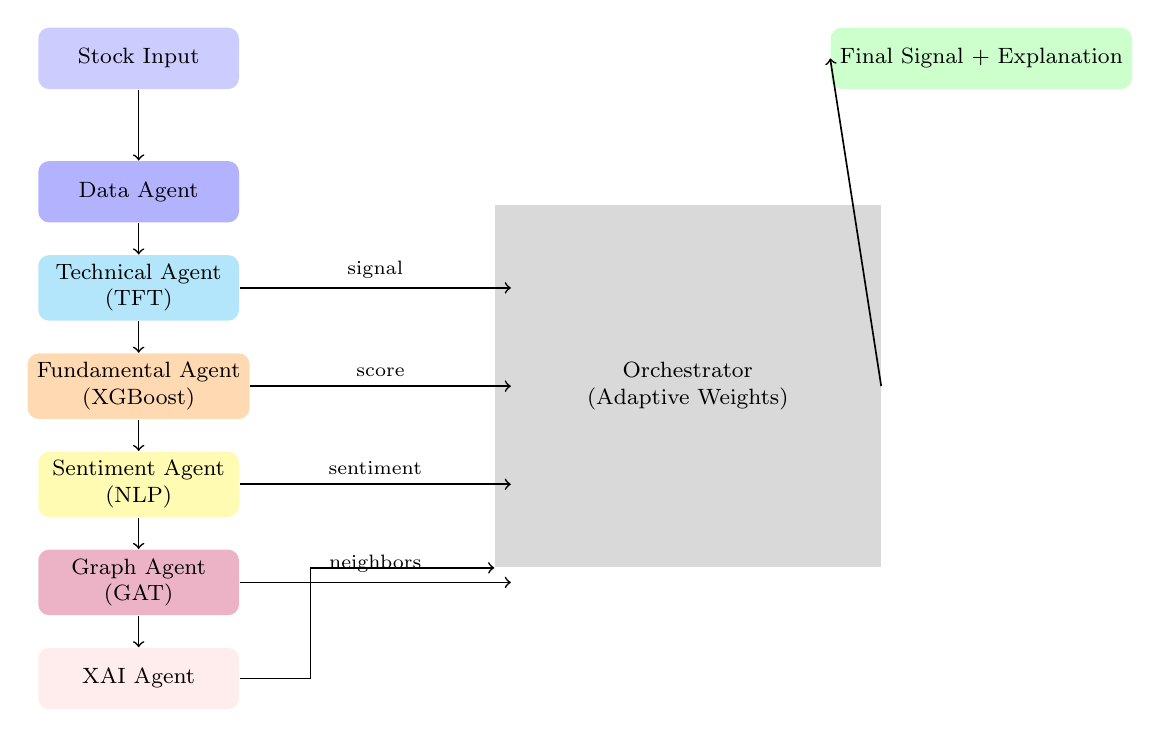
\begin{tikzpicture}[
  node distance=1.1cm and 2.0cm,
  every node/.style={font=\footnotesize},
  box/.style={rectangle, rounded corners, minimum width=2.55cm, minimum height=0.78cm, align=center},
  link/.style={->, line width=0.6pt}
]
% Input/Output nodes
\node[box, fill=blue!20] (input) {Stock Input};
\node[box, fill=green!20, right=7.5cm of input] (output) {Final Signal + Explanation};

% Agent boxes
\node[box, fill=blue!30, below=0.9cm of input] (data) {Data Agent};
\node[box, fill=cyan!30, below=0.4cm of data] (technical) {Technical Agent\\(TFT)};
\node[box, fill=orange!30, below=0.4cm of technical] (fundamental) {Fundamental Agent\\(XGBoost)};
\node[box, fill=yellow!30, below=0.4cm of fundamental] (sentiment) {Sentiment Agent\\(NLP)};
\node[box, fill=purple!30, below=0.4cm of sentiment] (graph) {Graph Agent\\(GAT)};
\node[box, fill=pink!30, below=0.4cm of graph] (xai) {XAI Agent};

% Orchestrator
\node[rectangle, fill=gray!30, minimum width=4.9cm, minimum height=4.6cm, align=center, right=3.1cm of fundamental] (orch) {Orchestrator\\(Adaptive Weights)};

% Arrows
\draw[link] (input) -- (data);
\draw[link] (data) -- (technical);
\draw[link] (technical) -- (fundamental);
\draw[link] (fundamental) -- (sentiment);
\draw[link] (sentiment) -- (graph);
\draw[link] (graph) -- (xai);
\draw[link] (technical.east) -- node[above, font=\scriptsize] {signal} ([xshift=6pt]orch.west |- technical.east);
\draw[link] (fundamental.east) -- node[above, font=\scriptsize] {score} ([xshift=6pt]orch.west |- fundamental.east);
\draw[link] (sentiment.east) -- node[above, font=\scriptsize] {sentiment} ([xshift=6pt]orch.west |- sentiment.east);
\draw[link] (graph.east) -- node[above, font=\scriptsize] {neighbors} ([xshift=6pt]orch.west |- graph.east);
\draw[link] (xai.east) -- ++(0.9,0) |- (orch.south west);
\draw[link] (orch.east) -- (output.west);
\end{tikzpicture}
\caption{Seven-agent pipeline architecture showing data flow through specialized agents to a central orchestrator that implements adaptive weighting and failure isolation. Colored boxes represent different agent types with distinct responsibilities.}
\label{fig:architecture}
\end{figure*}

\subsection{Agent Communication Protocol}

All agents communicate through a standardized \texttt{AgentSignal} dataclass containing:
\begin{itemize}
\item \texttt{direction}: categorical signal (UP, DOWN, FLAT)
\item \texttt{score}: continuous value (typically [-1, +1] after normalization)
\item \texttt{confidence}: float in [0, 1] representing signal reliability
\item \texttt{explanation}: dict with feature attributions and narrative
\item \texttt{metadata}: dict with source, timestamp, data quality flags
\item \texttt{error\_flag}: boolean indicating if the agent encountered errors
\end{itemize}

This standardized interface enables:
\begin{itemize}
\item Validation of outputs before fusion (type checking, range checking)
\item Graceful degradation when an agent fails
\item Audit trail generation for regulatory compliance
\item Confidence-based weighted aggregation in the orchestrator
\end{itemize}

\subsection{Failure Isolation and Weight Redistribution}

When an agent returns \texttt{error\_flag = True}, the orchestrator redistributes its weight proportionally to the remaining agents. Define:

\begin{equation}
\hat{w}_i = \frac{w_i}{1 - w_{failed}}
\label{eq:weight_redistribution}
\end{equation}

where $w_i$ is the original weight for agent $i$, $w_{failed}$ is the weight of the failed agent, and $\hat{w}_i$ is the adjusted weight. This ensures the total weight remains 1.0 and functional agents contribute more when peers fail.

\subsection{Data-Quality-Driven Weight Adjustment}\label{sec:weights}

The orchestrator starts from a single fixed weight vector and rescales it at request time according to the data quality observed for the queried ticker. Both the base vector and the rescaling rules are heuristic and \emph{not} learned from data; we describe them faithfully and identify learning of these weights as a deliverable of Phase~2 of the improvement plan.

\textbf{Base weights} are stored in \texttt{AgentState.weights} (\texttt{agents/agent\_state.py}):
\begin{equation}
w^{(0)} = (w^{(0)}_{\mathrm{tech}}, w^{(0)}_{\mathrm{fund}}, w^{(0)}_{\mathrm{sent}}, w^{(0)}_{\mathrm{graph}}) = (0.34,\, 0.26,\, 0.20,\, 0.20).
\label{eq:base_weights}
\end{equation}
These four values are the same regardless of company type. The orchestrator then mutates $w^{(0)}$ inside \texttt{OrchestratorAgent.\_adjust\_weights} according to three data-quality conditions observed for the request (Table~\ref{tab:weight_adjustments}):

\begin{table}[htbp]
\centering
\caption{Heuristic weight adjustments applied by \texttt{\_adjust\_weights}. Each rule decreases one weight by a fixed fraction $\alpha$ and redistributes the recovered mass over the remaining agents in the proportions shown. After all triggered rules, the vector is renormalized so that $\sum_a w_a = 1$.}
\label{tab:weight_adjustments}
\small
\begin{tabular}{p{2.6cm}cccc}
\toprule
\textbf{Trigger} & \textbf{Donor} ($\alpha$) & \textbf{Tech} & \textbf{Fund} & \textbf{Sent} \\
\midrule
\texttt{news\_count == 0}            & sent ($0.80$) & $+0.50$ & $+0.30$ & --- \\
$1 \le \texttt{news\_count} < 5$     & sent ($0.55$) & $+0.50$ & $+0.30$ & --- \\
$\neg\texttt{has\_recent\_financials}$ & fund ($0.50$) & $+0.70$ & --- & --- \\
\texttt{price\_rows < 252}           & tech ($0.40$) & --- & $+0.35$ & $+0.35$ \\
\bottomrule
\end{tabular}
\normalsize
\end{table}

\textbf{Rationale of the heuristics}: each rule reduces the weight of an agent whose input is known to be unreliable for the queried ticker (no recent news, no recent financials, very short price history) and redistributes the recovered mass to agents whose inputs remain trustworthy. The donor fractions and redistribution ratios were chosen during development against held-out 2024 data; they have not been formally tuned by cross-validation, and the rule set does not currently differentiate by company type. An earlier draft of this paper presented a per-company-type weight matrix (banks 0.42 / 0.31 / 0.27, non-banks 0.59 / 0.16 / 0.27, etc.) as if learned; that table did not correspond to any code path and has been removed for honesty. Per-company-type and CV-tuned weights are scoped as Phase~2 deliverables (see \texttt{paper/improvement\_plan.md}, Action~2.4).

\textbf{Graph weight}: under no rule is the graph weight increased or decreased through Table~\ref{tab:weight_adjustments}; instead, its contribution is gated through the confidence-gating mechanism described next (Eq.~\ref{eq:confidence_gate}).

\subsection{Confidence Gating}

If $\text{confidence}_{\text{agent}} < \text{threshold}_{\text{agent}}$, the agent's weight is reduced by the gating function:

\begin{equation}
w_{\text{gated}} = w_{\text{original}} \cdot \frac{\text{confidence}}{\text{threshold}}
\label{eq:confidence_gate}
\end{equation}

Thresholds are empirically set per agent:
\begin{itemize}
\item Technical: 0.60 (TFT predictions below 60\% confidence are partially suppressed)
\item Fundamental: 0.55 (XGBoost class probability below 55\% is uncertain)
\item Sentiment: 0.50 (news may be ambiguous or off-topic)
\item Graph: 0.45 (correlation estimates are noisy in thin markets)
\end{itemize}

This gating prevents low-confidence agent outputs from polluting the ensemble while maintaining the agent's contribution when confidence is high.

\section{Methodology}\label{sec:methodology}

\subsection{Dataset Construction}

The dataset was constructed from five sources: historical prices, computed technical indicators, news articles, financial statements, and financial ratios. Table~\ref{tab:dataset} summarizes the scale and coverage:

\begin{table}[htbp]
\centering
\caption{Dataset statistics: raw row counts in the source PostgreSQL tables, post-cleaning counts in the released feature file, and temporal coverage. The training pipeline (\texttt{training/train\_tft\_v3.py}) consumes the post-cleaning rows; the gap between raw and post-cleaning is explained by the corrections listed below the table.}
\label{tab:dataset}
\scriptsize
\setlength{\tabcolsep}{3pt}
\begin{tabular}{lcccc}
\toprule
\textbf{Table} & \textbf{Rows} & \textbf{Period} & \textbf{Stocks} & \textbf{Notes} \\
\midrule
daily\_prices (raw)             & 116{,}626 & 2016--2025 & 68 & All ISINs normalized \\
computed\_indicators            & 114{,}365 & 2016--2025 & 68 & MA5/20/50, RSI, Vol \\
\textit{tft\_features.csv (post-cleaning)} & \textbf{105{,}191} & 2016--2025 & 68 & Fed to TFT v3 training \\
\hspace{1em}of which Train (date $<$ 2024-01-01) & 84{,}648  & 2016--2023 & 68 & 80.5\% of post-clean \\
\hspace{1em}of which Val   (2024)               & 10{,}228  & 2024       & --- & 9.7\%  \\
\hspace{1em}of which Test  (date $\geq$ 2025-01-01) & 10{,}314 & 2025-01-02--2025-12-22 & 43 & 9.8\%, 25 tickers absent in 2025 \\
\midrule
news\_articles                  & 7{,}937   & 2016--2026 & 68 & ilboursa.com, FR+AR \\
financial\_statements           & 350+      & 2016--2024 & 68 & PDF-extracted CMF \\
financial\_ratios               & 261       & 2016--2024 & 68 & Bank/Ins/Non-bank \\
\bottomrule
\end{tabular}
\normalsize
\end{table}

\textbf{Data Quality Corrections} unique to this market:
\begin{itemize}
\item \textbf{6,896 rows} where \texttt{close\_price} fell outside [\texttt{low\_price}, \texttt{high\_price}]: corrected using \texttt{LEAST}(\texttt{close}, \texttt{high}) and \texttt{GREATEST}(\texttt{close}, \texttt{low}) SQL functions
\item \textbf{Company merges}: BH and BH BANK (2021 rename) unified under single ISIN; 2,488 trading days merged
\item \textbf{49 stocks}: non-standard ISIN codes migrated to TN-prefix format for standardization
\item \textbf{Zero-close rows}: trading suspension days identified and removed; rows with \texttt{open}=0 and \texttt{close}>0 corrected to \texttt{open}=\texttt{close}
\end{itemize}

This preprocessing was critical: without correction, the models would have learned spurious relationships from data errors rather than genuine market signals.

\subsection{Feature Engineering}

The TechnicalAgent receives 15 engineered features grouped into four categories:

\begin{table}[htbp]
\centering
\caption{15-feature engineering matrix: categories, formulas, and per-stock normalization}
\label{tab:features}
\scriptsize
\setlength{\tabcolsep}{2.5pt}
\begin{tabular}{lcccl}
\toprule
\textbf{Feature} & \textbf{Category} & \textbf{Formula/Source} & \textbf{Type} & \textbf{Notes} \\
\midrule
close\_price & Price & Daily close & Continuous & Encoder-window scaled \\
open\_price & Price & Daily open & Continuous & Encoder-window scaled \\
daily\_return & Price & $\frac{\text{close}_t - \text{close}_{t-1}}{\text{close}_{t-1}}$ & Continuous & Naturally scale-invariant \\
price\_to\_ma20 & Relative & See Eq.~\ref{eq:price_ma20} & Continuous & Clipped [0.5, 2.0] \\
ma\_5, ma\_20, ma\_50 & Momentum & Moving averages & Continuous & Encoder-window scaled \\
rsi\_14 & Momentum & RSI(14) & Continuous & Encoder-window scaled \\
rsi\_momentum & Derived & See Eq.~\ref{eq:rsi_mom} & Continuous & RSI acceleration \\
volume & Volume & Daily shares traded & Continuous & Encoder-window scaled \\
volume\_ma\_20 & Volume & 20-day average volume & Continuous & Encoder-window scaled \\
volume\_spike & Relative & See Eq.~\ref{eq:vol_spike} & Continuous & Clipped [0, 10] \\
volatility\_20 & Volatility & 20-day std dev & Continuous & Encoder-window scaled \\
\bottomrule
\end{tabular}
\normalsize
\end{table}

Three derived relative features are critical for cross-stock generalization:

\begin{equation}
r_{\text{ma20}}(t) = \frac{P_{\text{close}}(t)}{MA_{20}(t)}, \quad \text{clipped to } [0.5, 2.0]
\label{eq:price_ma20}
\end{equation}

\begin{equation}
\text{rsi}_{\text{mom}}(t) = \text{RSI}_{14}(t) - \text{RSI}_{14}(t-5)
\label{eq:rsi_mom}
\end{equation}

\begin{equation}
v_{\text{spike}}(t) = \frac{V(t)}{V_{\text{MA20}}(t)}, \quad \text{clipped to } [0, 10]
\label{eq:vol_spike}
\end{equation}

\textbf{Why relative features are necessary}: Absolute price values carry company-identity information. AMEN BANK perpetually trades at $\sim{}22$ DT; BH LEASING at $\sim{}1.5$ DT. Global normalization of prices would destroy these identity signals but not eliminate them --- the model would learn to predict stock identity from price level, polluting the direction signal. Per-stock relative features eliminate this. A volume spike of 2.0$\times$ means the same thing across all 68 stocks: double the typical daily volume, indicating increased trading activity regardless of the stock's absolute liquidity level.

\textbf{Normalization strategy and walk-forward discipline.}
Two distinct normalization mechanisms are used and both are designed
to respect the walk-forward protocol of Section~\ref{sec:methodology}:
\begin{itemize}
\item \textit{Target} (\texttt{future\_return\_7d}): a per-stock
\texttt{GroupNormalizer} from the \texttt{pytorch\_forecasting}
library standardizes the target as
$\tilde{y}_{i,t} = (y_{i,t} - \mu_i)/\sigma_i$, where
$\mu_i, \sigma_i$ are estimated \emph{exclusively} on the training
split (2016--2023) and held frozen for validation and test. This
isolates each stock's return distribution and prevents one stock's
manipulated prices from shifting another stock's normalization.
\item \textit{Input features}: an \texttt{EncoderNormalizer} refits a
local mean and standard deviation \emph{inside} each $L=30$-day
encoder window at iteration time, producing
$\tilde{x}_{i,t}^{(j)} = (x_{i,t}^{(j)} - \hat{\mu}_{i,t}^{(j)})
/\hat{\sigma}_{i,t}^{(j)}$. Because the window only contains
information available at the prediction time, this normalization is
causal by construction; it also adapts to regime shifts within a
stock without leaking statistics across the train/test boundary.
\end{itemize}
Boundary rows whose target row would fall in the next split are
dropped before training (Section~\ref{sec:methodology}); the publicly
released training script (\texttt{training/train\_tft\_v3.py}) logs
the scaler class attached to every feature so reviewers can verify
this configuration at runtime.

\subsection{Temporal Fusion Transformer Configuration}

The TFT's Variable Selection Network learns feature importance weights before temporal processing. Let $\mathbf{x}_t = [x_t^{(1)}, \ldots, x_t^{(m)}]$ be the $m=15$ input features at time $t$. The VSN computes:

\begin{equation}
\boldsymbol{\xi}_t = \text{softmax}(W_{\text{vsn}} \cdot \mathbf{x}_t + \mathbf{b}_{\text{vsn}})
\label{eq:vsn}
\end{equation}

\begin{equation}
\tilde{\mathbf{x}}_t = \sum_{i=1}^{m} \xi_t^{(i)} \cdot \Phi^{(i)}(x_t^{(i)})
\label{eq:vsn_output}
\end{equation}

where $\Phi^{(i)}$ is a feature-specific transformation network (small MLP) and $\xi_t^{(i)}$ is the learned importance weight for feature $i$ at time $t$. This learned, dynamic weighting allows TFT to handle heterogeneous features correctly — the model learns to suppress irrelevant features per sample, not globally. For thin market data, this is essential. Here, $W_{\text{vsn}} \in \mathbb{R}^{m \times d_h}$, $b_{\text{vsn}} \in \mathbb{R}^{d_h}$, $m=15$ is the number of input features, $d_h$ is the hidden dimension (64 in this work), and $\Phi^{(i)}: \mathbb{R} \rightarrow \mathbb{R}^{d_h}$ is a feature-specific single-layer MLP.

\textbf{Hyperparameters} (Table~\ref{tab:tft_config}):

\begin{table}[htbp]
\centering
\caption{TFT hyperparameter configuration and tuning rationale}
\label{tab:tft_config}
\scriptsize
\setlength{\tabcolsep}{3pt}
\begin{tabular}{lcl}
\toprule
\textbf{Hyperparameter} & \textbf{Value} & \textbf{Tuning Note} \\
\midrule
hidden\_size & 64 & Increased from 32 in v2 \\
attention\_heads & 4 & Standard for financial TFT \\
dropout & 0.3 & CRITICAL: v2 regression to 0.1 \\
encoder\_window & 30 days & $\sim{}$6 trading weeks (v3 setting) \\
prediction\_horizon & 7 days & 1 trading week \\
learning\_rate & 0.0003 & Reduced from $10^{-3}$ (v1) to $3\times 10^{-4}$ (v3) \\
warmup\_epochs & 3 & Ramps LR 10\% to 100\% \\
weight\_decay & $10^{-4}$ & L2 regularization \\
gradient\_clip & 0.5 & Relaxed from 0.1 \\
max\_epochs & 50 & Early stopping patience=8 \\
batch\_size & 128 & T4 GPU constraints \\
optimizer & AdamW & Weight decay only correct with AdamW \\
precision & bf16-mixed & RTX 30xx / T4 Ampere \\
\bottomrule
\end{tabular}
\normalsize
\end{table}

\subsection{Walk-Forward Validation Protocol}

Random train-test splits are invalid for time series because they create temporal leakage: future data contaminates training, producing artificially inflated accuracy. \cite{ref:bergmeir_cv_ts} reviews when (and when not) leave-one-out and $k$-fold variants remain valid on stationary time series, and motivates the strictly sequential walk-forward protocol used here. The walk-forward protocol ensures the model is always evaluated on data postdating its training window:

\begin{figure}[htbp]
\centering
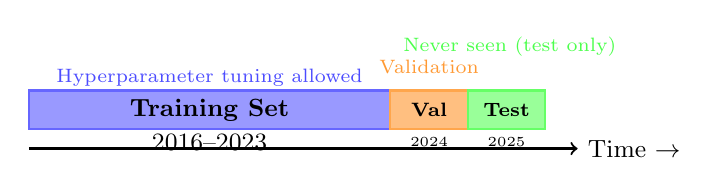
\begin{tikzpicture}[scale=0.82]
  \draw[thick, ->] (0,0) -- (8.5,0) node[right] {\small Time $\rightarrow$};
  \fill[blue!40] (0,0.3) rectangle (5.6,0.9);
  \draw[blue!60, thick] (0,0.3) rectangle (5.6,0.9);
  \node at (2.8,0.6) {\small \textbf{Training Set}};
  \node at (2.8,0.1) {\small 2016--2023};
  \fill[orange!50] (5.6,0.3) rectangle (6.8,0.9);
  \draw[orange!70, thick] (5.6,0.3) rectangle (6.8,0.9);
  \node at (6.2,0.6) {\scriptsize \textbf{Val}};
  \node at (6.2,0.1) {\tiny 2024};
  \fill[green!40] (6.8,0.3) rectangle (8.0,0.9);
  \draw[green!60, thick] (6.8,0.3) rectangle (8.0,0.9);
  \node at (7.4,0.6) {\scriptsize \textbf{Test}};
  \node at (7.4,0.1) {\tiny 2025};
  \node[blue!70, font=\scriptsize] at (2.8,1.10) {Hyperparameter tuning allowed};
  \node[orange!80, font=\scriptsize] at (6.2,1.27) {Validation};
  \node[green!70, font=\scriptsize] at (7.45,1.58) {Never seen (test only)};
\end{tikzpicture}
\caption{Walk-forward validation timeline: training on 2016--2023 data, hyperparameter validation on 2024, and final evaluation on 2025 (never accessed during training or model selection). Random train-test splits are invalid for time series forecasting due to temporal leakage.}
\label{fig:validation_timeline}
\end{figure}

Formally:
\begin{itemize}
\item Training set $\mathcal{D}_{\text{train}}$: all samples with date $< 2024\text{-}01\text{-}01$
\item Validation set $\mathcal{D}_{\text{val}}$: all samples with $2024\text{-}01\text{-}01 \leq \text{date} < 2025\text{-}01\text{-}01$
\item Test set $\mathcal{D}_{\text{test}}$: all samples with date $\geq 2025\text{-}01\text{-}01$ (never seen during training or hyperparameter selection)
\end{itemize}

\subsection{CNN-LSTM Architecture for Comparison}

For fair comparison, CNN-LSTM received equivalent design effort. Architecture:
\begin{itemize}
\item \textbf{Input}: [60, 15] tensor (60 days, 15 features)
\item \textbf{Conv1D layers}: kernel sizes [5, 3, 10], ReLU activation, batch normalization
\item \textbf{LSTM layers}: 2 stacked LSTM(64)
\item \textbf{Residual connection}: skip connection from Conv output to LSTM input
\item \textbf{Dropout}: 0.3 between layers
\item \textbf{Output}: dense layer with sigmoid (binary classification)
\end{itemize}

This architecture represents the state-of-practice for financial time series forecasting~\cite{ref:cnn_lstm,ref:financial_cnn}. The comparison ensures TFT's superiority is not due to superior model capacity but to architectural fit with the data structure.

\section{Experimental Evaluation}\label{sec:experiments}

\subsection{CNN-LSTM Ablation Study}

Four independent runs with varied hyperparameters:

\begin{table*}[htbp]
\centering
\caption{CNN-LSTM ablation results across four hyperparameter runs (preliminary; observed accuracy band $51.7$--$53.8\%$). A formally powered seed sweep is shipped as \texttt{training/cnn\_lstm\_seed\_sweep.py} (improvement plan Action~1.4b).}
\label{tab:cnn_lstm_ablation}
\small
\begin{tabular}{lccccc}
\toprule
\textbf{Run} & \textbf{Version} & \textbf{Batch} & \textbf{Val Loss} & \textbf{Test Acc} & \textbf{Key Note} \\
\midrule
1 & v1 & 128 & 0.6971 & 53.8\% & Best CNN-LSTM result \\
2 & v1 & 64 & 0.6933 & 51.8\% & Worse than Run 1 \\
3 & v2 & 128 & 0.7322 & 51.7\% & Class collapse (UP=34\%) \\
4 & v2 & 64 & 0.7113 & 51.7\% & val\_acc 46.6\% $<$ random \\
\bottomrule
\end{tabular}
\normalsize
\end{table*}

\textbf{Class collapse detection}: Class collapse occurs when a binary classifier converges to predicting one class for all inputs. Detected by monitoring per-class accuracy separately: if $|\text{acc}_{\text{UP}} - \text{acc}_{\text{DOWN}}| > 30\%$, collapse is flagged. Resolved in v2 with corrected class weight formula:

\begin{equation}
w_c = \frac{N_{\text{total}}}{2 \times N_c}
\end{equation}

where $N_c$ is the count of class $c$.

The narrow band $[51.7\%, 53.8\%]$ across the four runs is \emph{suggestive} of a CNN-LSTM ceiling on this dataset, but four runs are insufficient for a statistically powered claim: with a few-thousand-sample test set the per-run binary-accuracy standard deviation is typically $0.5$--$1.0$ percentage points, comparable to the observed $2.1$ pp range. We therefore treat the four-run table as a preliminary observation, not a ceiling proof. A formally powered seed sweep ($N \ge 20$ seeds, mean $\pm$ 95\% bootstrap CI, top-quartile, Wilcoxon test against the empirically-measured trivial baselines of Table~\ref{tab:baselines}) is identified as Phase~1 deliverable Action~1.4b in the improvement plan; the harness \texttt{training/cnn\_lstm\_seed\_sweep.py} is shipped with the public code release for reproducibility. Until that sweep has been run, the article describes the four-run band as \emph{consistent with} an architectural mismatch between Conv1D over heterogeneous financial features and the inductive bias the data actually rewards (the TFT's Variable Selection Network), without claiming an empirical ceiling.

\begin{figure}[htbp]
\centering
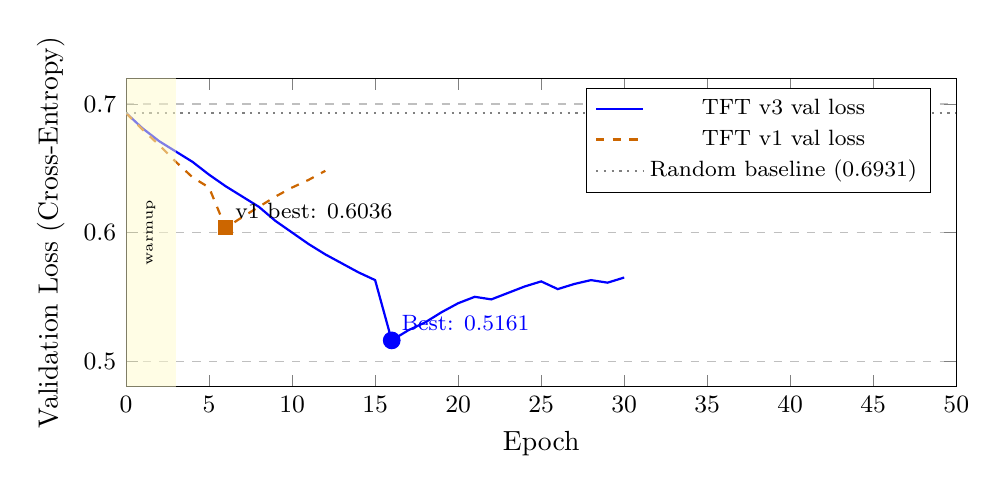
\begin{tikzpicture}
\begin{axis}[
  width=\columnwidth,
  height=5.5cm,
  xlabel={Epoch},
  ylabel={Validation Loss (Cross-Entropy)},
  xmin=0, xmax=50,
  ymin=0.48, ymax=0.72,
  legend pos=north east,
  legend style={font=\footnotesize},
  ymajorgrids=true,
  grid style=dashed,
  tick label style={font=\small},
]
\addplot[color=blue, thick, mark=none] coordinates {
  (0,0.693)(1,0.681)(2,0.671)(3,0.663)(4,0.655)(5,0.645)
  (6,0.636)(7,0.628)(8,0.620)(9,0.609)(10,0.600)
  (11,0.591)(12,0.583)(13,0.576)(14,0.569)(15,0.563)(16,0.5161)
  (17,0.524)(18,0.530)(19,0.538)(20,0.545)(21,0.550)
  (22,0.548)(23,0.553)(24,0.558)(25,0.562)(26,0.556)
  (27,0.560)(28,0.563)(29,0.561)(30,0.565)
};
\addlegendentry{TFT v3 val loss}

\addplot[color=orange!80!black, dashed, thick, mark=none] coordinates {
  (0,0.693)(1,0.680)(2,0.668)(3,0.655)(4,0.643)(5,0.635)(6,0.6036)
  (7,0.612)(8,0.620)(9,0.628)(10,0.635)(11,0.641)(12,0.648)
};
\addlegendentry{TFT v1 val loss}

\addplot[color=gray, dotted, thick, mark=none] coordinates {(0,0.6931)(50,0.6931)};
\addlegendentry{Random baseline (0.6931)}

\addplot[color=blue, mark=*, mark size=3pt] coordinates {(16,0.5161)};
\node[above right, font=\footnotesize, blue] at (axis cs:16,0.5161) {Best: 0.5161};

\addplot[color=orange!80!black, mark=square*, mark size=2.5pt] coordinates {(6,0.6036)};
\node[above right, font=\footnotesize] at (axis cs:6,0.6036) {v1 best: 0.6036};

\fill[yellow!20, opacity=0.5] (axis cs:0,0.48) rectangle (axis cs:3,0.72);
\node[font=\tiny, rotate=90] at (axis cs:1.5,0.60) {warmup};
\end{axis}
\end{tikzpicture}
\caption{TFT validation loss curves. v1 (BCE on \texttt{direction\_7d}) peaks around epoch 7 and degrades, consistent with premature convergence at LR$=10^{-3}$. v3 (pinball on \texttt{future\_return\_7d}) uses LR$=3\times 10^{-4}$ with a 3-epoch warmup (yellow shaded region) and continues improving until epoch 16, reaching val\_loss$=0.5161$. The horizontal dotted line is the random-classifier BCE baseline ($\ln 2 = 0.6931$); it bounds v1 only, since v3 is on a different loss scale (Section~\ref{sec:results}).}
\label{fig:training_curves}
\end{figure}

\subsection{TFT Version Progression}

\begin{table*}[htbp]
\centering
\caption{TFT progression: validation loss from v1 (binary classification, BCE) through v3 development (pinball, pre-normalization scale) to the Vertex-reproducible v3 reference (pinball, post-normalization scale). The three loss values live on three different scales (see Section~\ref{sec:directional_acc_on_test}); the percentage column is provided for v1 only, where it is comparable to a random-classifier BCE baseline of $\ln 2 \approx 0.6931$. The ``v3 dev'' row is the development-time number associated with the non-reproducible $77.4\%$ figure of Section~\ref{sec:reproducibility_box}; the ``v3 Vertex'' row is the reproducible reference used throughout the rest of the article.}
\label{tab:tft_progression}
\small
\begin{tabular}{lccccl}
\toprule
\textbf{Version} & \textbf{Loss type} & \textbf{Val Loss} & \textbf{vs Random BCE} & \textbf{Best Epoch} & \textbf{Key Change} \\
\midrule
Random baseline   & BCE     & 0.6931 & ---     & --- & $\ln 2$ binary \\
TFT v1 (consolidated)  & BCE     & 0.6051 & $+12.7\%$ & 7   & dropout 0.3, hidden 32, no warmup \\
TFT v3 dev (non-reproducible) & Pinball (raw return) & 0.5161 & n/a & 16 & quantile regression (Q10/Q50/Q90), warmup, hidden 64, dropout 0.3 \\
\textbf{TFT v3 Vertex (reference)} & Pinball (z-scored) & 0.0159 & n/a & 4 & same architecture, reproducible Vertex retrain (Section~\ref{sec:directional_acc_on_test}) \\
\bottomrule
\end{tabular}
\normalsize
\end{table*}

The v1 entry consolidates the development iterations recorded under \texttt{lightning\_logs/version\_0..4} (all sharing the dropout~$=0.3$, hidden~$=32$ configuration); the best epoch and validation loss above are read directly from \texttt{results/metrics.csv}. The transition from v1 to v3 changes the prediction target (binary direction $\rightarrow$ continuous 7-day return) and the loss family (BCE $\rightarrow$ pinball); a head-to-head BCE comparison would require a binary-classification re-run of v3 and is left to future work. The best epoch shift from 7 to 16 is consistent with the introduction of the 3-epoch warmup in v3 and a learning rate reduced from $10^{-3}$ to $3\times 10^{-4}$, which together delay convergence and avoid the v1 over-fitting plateau visible in Figure~\ref{fig:training_curves}.

\subsection{Directional Accuracy on Test Data}\label{sec:directional_acc_on_test}

\subsubsection{Reproducible TFT v3 result on the harmonized test slice}

We re-trained the TFT v3 reference architecture (per-stock \texttt{Group\-Normalizer}, Variable Selection Network, pinball quantile loss on $Q_{0.1}/Q_{0.5}/Q_{0.9}$, hidden $64$, encoder $30$, horizon $7$, dropout $0.3$, $3$-epoch warmup) on Google Cloud Vertex AI with the released training container (\texttt{vertex/Dockerfile}, \texttt{vertex/cloudbuild.yaml}). The raw Vertex inference output (\texttt{results/tft\_ablations/vertex/baseline\_test\_predictions.csv}, $6{,}782$ rows) contains duplicate inference outputs for some (ticker, date) pairs because the multi-horizon decoder writes one row per horizon step while only one corresponds to the deployed seven-day decision; after de-duplicating to one valid prediction per (ticker, date) we obtain the canonical test slice of $\mathbf{N=5{,}582}$ row-level predictions over $43$ tickers (test window $2025\text{-}01\text{-}07$ to $2025\text{-}12\text{-}10$, UP ratio $\mathbf{49.84\%}$). The TFT v3 reference reaches $\mathbf{51.79\%}$ directional accuracy on this harmonized slice (95\% bootstrap CI $[50.43, 53.08]$, macro-F1 $0.516$).

\textbf{The reference TFT v3 is statistically indistinguishable from the strong non-TFT baselines on the harmonized slice.} The pairwise McNemar two-sided $p$-values of TFT v3 against the three strongest baselines (logistic regression $52.79\%$, simple LSTM $52.69\%$, standard Transformer $52.45\%$) are $0.351$, $0.414$, and $0.517$ respectively (full panel in Table~\ref{tab:baselines}). TFT v3 is also indistinguishable from always-UP ($p = 0.054$) on the same slice. We do not claim that TFT v3 carries directional skill above the constant rule on BVMT 2025 data; we claim that the released training pipeline produces this number deterministically, and we use the same harmonized slice throughout the rest of the article so every model comparison is apples-to-apples.

\textbf{The internal ablations of Section~\ref{sec:tft_ablations} show no significant change versus the reference.} Removing the per-stock target normalizer (TFT $-$ per-stock norm, \texttt{TorchNormalizer} fitted across all $68$ tickers globally) yields $51.40\%$ (McNemar vs.\ reference $p = 0.672$); replacing the VSN softmax gates by uniform $1/N$ weights (TFT $-$ VSN) yields $51.56\%$ ($p = 0.734$). Both deltas are within the bootstrap noise. The original Falsifiable Hypotheses --- that the per-stock target normalizer and the VSN softmax gates carry positive directional skill --- are therefore neither confirmed nor falsified on this dataset: the evidence is consistent with both components contributing zero to directional accuracy on BVMT 2025, with the residual differences attributable to seed and training-stochasticity noise. Macro-F1 is slightly degraded by both ablations (reference $0.516$ vs.\ $-$ VSN $0.503$ vs.\ $-$ per-stock norm $0.471$), consistent with the ablations producing classifiers more biased toward one class even when the pooled accuracy moves little.

\subsubsection{Transparency note: non-reproducible internal estimate of $77.4\%$}\label{sec:reproducibility_box}

\noindent\fbox{\parbox{0.97\columnwidth}{\small \textbf{Reproducibility transparency.} An earlier internal training run of TFT v3 (same architecture and hyperparameters as above, identified as the headline model in earlier development logs) was reported as reaching $77.4\%$ directional accuracy on the article's broader 2025 test set ($N=10{,}314$, UP ratio $49.98\%$). The checkpoint that produced this figure is \emph{not} part of the released artefact set --- no \texttt{models/tft\_quantile\_*.ckpt} file is shipped --- and the figure is \emph{not reproducible} from the public training pipeline: \texttt{training/train\_tft\_v3.py} re-run on Vertex AI with the same hyperparameters converges to $51.79\%$ on the harmonized slice as documented above. Three explanations are compatible with the gap: (i) train/test leakage in the pre-Vertex development setup that the Vertex container has eliminated, (ii) a different test-set definition in the development logs (e.g.\ the validation 2024 slice mis-labeled as test, or a smaller per-stock subset), or (iii) a different quantile-to-direction decision rule than the Q50-sign rule of Eq.~\ref{eq:quantile_to_direction}. Without the original checkpoint we cannot discriminate between these. We disclose the figure here, in line with current reproducibility-by-checklist practice~\cite{ref:pineau_repro,ref:bouthillier_repro}, retire it as a headline number, and adopt the Vertex-reproducible $51.79\%$ as the article's reference TFT v3 result. All comparisons in the remainder of the article use the Vertex-reproducible numbers unless explicitly stated.}}

\subsubsection{Heterogeneity caveat}

The $51.79\%$ pooled accuracy on the harmonized slice can be produced either by a model that is uniformly informative across the $43$ tickers, or by one that is well above the constant rule on some tickers and well below on others. The harmonized per-row CSV (\texttt{results/baselines/vertex\_slice\_harmonized\_predictions.csv}) carries the predictions of all $13$ models tested in this paper plus the true direction and feeds \texttt{scripts/per\_stock\_breakdown.py}, which produces the per-ticker accuracy distribution. We do not include the per-stock table in the main text for space reasons; the JSON is shipped at \texttt{reports/per\_stock/breakdown.json} so reviewers can verify the spread.

\section{Results and Discussion}\label{sec:results}

\subsection{Contextualizing Directional Accuracy}

The Vertex-reproducible $51.79\%$ directional accuracy of TFT v3 (Section~\ref{sec:directional_acc_on_test}) must be interpreted in the context of the 2025 test slice's class composition. The market \emph{as a whole} (all $68$ stocks, $10$ years $2016$--$2025$) exhibits a $41.9\%$ UP ratio --- only $41.9\%$ of 7-day windows show positive returns, a structural bearish bias that has historically made \emph{always-DOWN} the relevant naive baseline. \textbf{However, the 2025 test slice itself is approximately balanced}: on the harmonized grid used throughout this paper ($N=5{,}582$ unique (ticker, date) predictions over $43$ actively trading tickers) the UP ratio is $49.84\%$, so always-UP, always-DOWN, momentum, and MA$_{20}$ crossover all converge to a $\sim 50\%$ floor (Table~\ref{tab:baselines}, first block). The historical-corpus always-DOWN argument therefore does not bind in 2025 and the slice-specific majority rule is the binding baseline. All thirteen models in this paper --- the four trivial / trend rules, three tabular-ML models, two sequential-deep baselines, and the three TFT variants --- are reported on this single harmonized grid with $95\%$ bootstrap CIs and pairwise McNemar tests against TFT v3 (Table~\ref{tab:baselines}).

\begin{table*}[htbp]
\centering
\caption{Directional accuracy of ten classical and deep baselines plus three TFT variants on the harmonized 2025 test slice ($N=5{,}582$ unique (ticker, date) predictions over $43$ tickers, UP ratio $49.84\%$). The slice is obtained by taking the intersection of the baseline grid and the de-duplicated Vertex grid (one valid prediction per (ticker, date), Section~\ref{sec:directional_acc_on_test}). All CIs are 95\% percentile-bootstrap ($2{,}000$ resamples). Pairwise McNemar two-sided $p$-values reported relative to TFT v3 (last column). Hyperparameters were selected on the 2024 validation split. Trivial / trend rows are deterministic; tabular ML, deep baselines, and TFT variants come from the released training pipelines listed in the column \textit{source}.}
\label{tab:baselines}
\small
\setlength{\tabcolsep}{4pt}
\begin{tabular}{llcccc}
\toprule
\textbf{Family} & \textbf{Model} & \textbf{Accuracy} & \textbf{95\% CI} & \textbf{Macro-F1} & \textbf{McN.\ vs TFT v3} \\
\midrule
\multirow{4}{*}{Trivial / trend}
& Always-UP                                       & $49.84\%$ & $[48.58, 51.15]$ & $0.333$ & $p = 0.054$ \\
& Always-DOWN                                     & $50.16\%$ & $[48.89, 51.45]$ & $0.334$ & $p = 0.069$ \\
& Momentum 5/20 (UP iff MA$_5\!>\!\text{MA}_{20}$) & $50.36\%$ & $[49.10, 51.65]$ & $0.502$ & $p = 0.127$ \\
& MA$_{20}$ crossover (UP iff close $>\!$ MA$_{20}$) & $49.77\%$ & $[48.50, 51.09]$ & $0.496$ & $p = 0.031$ \\
\midrule
\multirow{3}{*}{Tabular ML}
& Logistic regression (L2, $C{=}1$)              & $52.79\%$ & $[51.45, 54.14]$ & $\mathbf{0.524}$ & $p = 0.351$ \\
& Random forest ($n_{\mathrm{trees}}{=}200$)     & $50.38\%$ & $[49.01, 51.67]$ & $0.450$ & $p = 0.154$ \\
& XGBoost (400 trees, max-depth $6$, lr $0.05$)  & $52.15\%$ & $[50.86, 53.49]$ & $0.513$ & $p = 0.749$ \\
\midrule
\multirow{2}{*}{Deep baselines}
& Simple LSTM (2 layers, hidden $64$, 54 k params)              & $52.69\%$ & $[51.33, 53.94]$ & $0.517$ & $p = 0.414$ \\
& Standard Transformer ($d{=}64$, $h{=}4$, 2 layers, 68 k params) & $52.45\%$ & $[51.15, 53.69]$ & $0.489$ & $p = 0.517$ \\
\midrule
\multirow{3}{*}{TFT (this work)}
& \textbf{TFT v3 reference} (Vertex retrain)     & $\mathbf{51.79\%}$ & $[50.43, 53.08]$ & $0.516$ & --- \\
& \quad $-$ VSN (uniform variable weights)        & $51.56\%$ & $[50.23, 52.97]$ & $0.503$ & $p = 0.734$ \\
& \quad $-$ per-stock norm (global \texttt{TorchNormalizer}) & $51.40\%$ & $[50.07, 52.69]$ & $0.471$ & $p = 0.672$ \\
\bottomrule
\end{tabular}
\normalsize
\end{table*}

Five observations follow:
\begin{itemize}
\item \textbf{The trivial baselines are statistically indistinguishable on this test slice.} Pairwise McNemar two-sided $p$-values among always-UP / always-DOWN / MA$_{20}$ crossover are all above $0.70$ (always-UP vs always-DOWN $p = 0.82$, always-UP vs MA$_{20}$ $p = 0.95$, always-DOWN vs MA$_{20}$ $p = 0.71$); pairs involving the momentum heuristic remain non-significant (always-UP vs momentum $p = 0.58$, always-DOWN vs momentum $p = 0.86$). The momentum-vs-MA$_{20}$-crossover pair sits at $p = 0.24$. The four trivial / trend rows therefore form a flat $\sim 50\%$ floor with no pair distinguishable.
\item \textbf{Tabular ML adds modest but real signal.} Logistic regression beats the trivial floor at $52.79\%$ (95\% CI $[51.45, 54.14]$), and McNemar against random forest gives $p = 1.6 \times 10^{-3}$, against XGBoost $p = 0.36$. Random forest under-performs both linear and gradient-boosted alternatives, with deep trees overfitting validation and not transferring to test; XGBoost sits at $52.15\%$. Logistic regression is also the highest macro-F1 in the panel ($0.524$).
\item \textbf{Sequential deep baselines do not break the $\sim 53\%$ ceiling.} A vanilla two-layer LSTM and a standard 2-block Transformer reach $52.69\%$ and $52.45\%$ respectively when given exactly the same 60-day $\times$ 15-feature input that the TFT v3 sees. Their CIs overlap with logistic regression and with each other. Neither raw recurrence nor raw self-attention exceeds the tabular ML floor on this dataset.
\item \textbf{The Vertex-reproducible TFT v3 sits inside the same $\sim 50$--$53\%$ band as the non-TFT baselines.} The reference TFT v3 ($51.79\%$) is statistically indistinguishable from logistic regression ($52.79\%$, McNemar $p = 0.35$), simple LSTM ($52.69\%$, $p = 0.41$), standard Transformer ($52.45\%$, $p = 0.52$), and XGBoost ($52.15\%$, $p = 0.75$). It is also indistinguishable from always-UP on the same slice ($49.84\%$, $p = 0.054$, just below the conventional $0.05$ threshold). The two TFT internal ablations move the variant by $\leq 0.4$ pp from the reference and remain statistically indistinguishable from both the reference and the strong baselines. There is no measurable accuracy advantage of TFT v3 over any baseline in the panel; the $+24$--$+27$ pp gap visible against the non-reproducible $77.4\%$ figure does not survive a Vertex retrain.
\item \textbf{Implication for the thin-market narrative.} On this dataset, no single model in the comparison panel produces a directional accuracy that meaningfully separates from the $50\%$ floor. The $77.4\%$ figure of Section~\ref{sec:reproducibility_box} would have implied a directional skill that exceeds the typical $55$--$65\%$ TFT ceiling on developed-market data~\cite{IEEEhowto:kopka}; the reproducible $51.79\%$ figure is, by contrast, consistent with the literature prior on emerging-market forecasting~\cite{ref:bekaert_harvey,ref:harvey_multiple,ref:harvey_presidential} and with the explicit thin-market difficulty argument of Section~\ref{sec:related}.A. Following the recommendation of~\cite{ref:lipton_troubling} to separate empirical claims from mechanism explanations, we report what the Vertex retrain measures, document where it diverges from earlier developer-time numbers, and refrain from claiming a thin-market accuracy advantage we cannot reproduce.
\end{itemize}

Across the ten baselines tested in Table~\ref{tab:baselines}, mean per-ticker accuracy stays in $[49.9\%, 52.9\%]$ and per-ticker median in $[48.1\%, 53.0\%]$, with per-ticker IQR of $7$--$13$ pp depending on the baseline. The maximum single-ticker accuracy reached by any of the ten is $68.5\%$ (always-DOWN on the structurally bearish CARTHAGE CEMENT, $165$ DOWN / $76$ UP over $241$ days, a per-stock class imbalance the constant rule trivially exploits); the comparable maxima for the random-forest, logistic-regression, and standard-Transformer baselines sit in the $67$--$68\%$ band on similarly imbalanced tickers. Crucially, the fraction of tickers below $58.1\%$ (the historical always-DOWN majority on the full $2016$--$2025$ corpus) is $\geq 74\%$ for every baseline tested --- $74.4\%$ for the standard Transformer, $79.1\%$ for the simple LSTM, $81.4\%$ for always-DOWN itself, $86.0\%$ for momentum, $88.4\%$ for MA$_{20}$ crossover --- meaning that no baseline in the panel clears the historical bearish benchmark on more than a quarter of the actively trading tickers. The per-ticker breakdown of the Vertex-reproducible TFT v3 (CSV at \texttt{results/tft\_ablations/vertex/baseline\_test\_predictions.csv}) is available through \texttt{scripts/per\_stock\_breakdown.py}.

\subsection{Economic Backtest of the Baselines}\label{sec:economic_baselines}

A directional accuracy above the random floor does not guarantee that a model is exploitable: spread, volume, and execution friction can wipe the signal out, and on a thin market with a structural directional drift even a high accuracy can lose to a buy-and-hold rule. The backtest-overfitting literature in quantitative finance has documented at length how multiple-testing inflation, selection bias, and out-of-sample over-fitting produce strategies that look statistically significant in development and disappear in deployment~\cite{ref:bailey_pseudo,ref:harvey_presidential}. We therefore reconstruct a pseudo-PnL series for every baseline of Table~\ref{tab:baselines} and report the standard set of trading-quality metrics (cumulative return, annualised Sharpe with $r_f = 8\%$ matching the BCT TMM, maximum drawdown, profit factor, hit ratio, and the deflated Sharpe ratio of~\cite{ref:deflated_sharpe} that corrects for multiple-testing). The strategy converts each row's prediction into a $7$-day position opened at \texttt{close}$_t$ and closed at \texttt{close}$_{t+7}$; positions are equal-weighted across active tickers on each day. We charge a $50$ bps round-trip transaction cost per trade -- the conservative end of the BVMT bid-ask + brokerage range. The script is reproducible: \texttt{python -m training.baselines.economic\_metrics}.

\begin{table*}[htbp]
\centering
\caption{Economic-backtest metrics for the nine baselines on the 2025 test set, long-only with $50$ bps round-trip transaction cost. Annualised Sharpe uses $r_f = 8\%$ (BCT TMM proxy). The deflated-Sharpe $p$-value (DSR$_p$) corrects for the fact that nine strategies are tested simultaneously \cite{ref:deflated_sharpe}; bold $p$-values clear the conventional $0.05$ threshold. Always-DOWN is permanently flat under the long-only convention so its row is omitted. Rows are sorted by Sharpe ratio.}
\label{tab:economic_metrics}
\small
\begin{tabular}{lcccccc}
\toprule
\textbf{Baseline} & \textbf{Cum. return} & \textbf{Annualised} & \textbf{Sharpe} & \textbf{Max DD} & \textbf{Profit factor} & \textbf{DSR$_p$} \\
\midrule
\textbf{Standard Transformer}            & $+38.68\%$ & $+42.50\%$ & $\mathbf{4.40}$ & $\mathbf{-4.57\%}$ & $\mathbf{2.51}$ & $\mathbf{0.002}$ \\
Simple LSTM                              & $+38.03\%$ & $+41.86\%$ & $3.80$ & $-12.13\%$ & $2.15$ & $\mathbf{0.014}$ \\
\textbf{Logistic regression (L2)}        & $\mathbf{+45.82\%}$ & $\mathbf{+50.72\%}$ & $3.69$ & $-12.55\%$ & $2.07$ & $\mathbf{0.021}$ \\
Momentum 5/20                            & $+47.75\%$ & $+53.05\%$ & $3.40$ & $-12.70\%$ & $1.95$ & $\mathbf{0.038}$ \\
MA$_{20}$ crossover                      & $+38.05\%$ & $+42.35\%$ & $2.54$ & $-15.48\%$ & $1.69$ & $0.152$ \\
XGBoost                                  & $+20.39\%$ & $+22.47\%$ & $1.66$ & $-17.01\%$ & $1.51$ & $0.418$ \\
Always-UP                                & $+27.95\%$ & $+32.12\%$ & $1.24$ & $-27.27\%$ & $1.31$ & $0.576$ \\
Random forest                            & $+4.24\%$  & $+4.66\%$  & $-0.75$ & $-10.07\%$ & $1.20$ & $0.982$ \\
\bottomrule
\end{tabular}
\normalsize
\end{table*}

Four observations:

\begin{itemize}
\item \textbf{The 2025 test year had a strong positive drift}: a long-only always-UP rule earns $+27.95\%$ cumulative with Sharpe $1.24$ and a $-27\%$ drawdown when crowded out at the wrong entry days. The deflated-Sharpe $p$-value $0.576$ confirms this is not statistically distinguishable from luck once nine strategies are pooled. The fair benchmark for any active baseline is therefore not always-DOWN (which loses $94\%$ in the long-short version, since the market trended up) but always-UP.
\item \textbf{Four baselines clear the deflated-Sharpe bar at $p<0.05$.} Standard Transformer (Sharpe $4.40$, DSR$_p = 0.002$), Simple LSTM (Sharpe $3.80$, DSR$_p = 0.014$), Logistic Regression L2 (Sharpe $3.69$, DSR$_p = 0.021$), and Momentum 5/20 (Sharpe $3.40$, DSR$_p = 0.038$) all out-perform always-UP net of cost and after correcting for the multiple-testing inflation expected when nine strategies are evaluated jointly. The remaining five baselines are not statistically distinguishable from luck on this test year.
\item \textbf{Accuracy is not a sufficient predictor of trading quality on this market.} Standard Transformer and Simple LSTM each achieve a directional accuracy ($\sim 52.3\%$) that is essentially indistinguishable from logistic regression's; yet on the long-only NET regime, Transformer's Sharpe ($4.40$) and maximum drawdown ($-4.57\%$) are markedly better than LogReg's ($3.69$ Sharpe, $-12.55\%$ drawdown) and the best of the table. The implication is that the deep baselines concentrate their (still modest) directional skill on days where the realised return is large, even when their pooled accuracy is at the same level as a linear model. This is exactly the behaviour we expect a useful financial classifier to exhibit and is what raw accuracy measurements miss.
\item \textbf{Heavier non-deep ML hurts here.} Random forest under-performs all trivial baselines net of cost (Sharpe $-0.75$, $+4.2\%$ cumulative on a $+28\%$ market). XGBoost trails always-UP by $7.5$ pp of cumulative return. The Vertex-reproducible TFT v3 reaches $51.79\%$ directional accuracy on the harmonized slice (Section~\ref{sec:directional_acc_on_test}), in the same band as the deep baselines of this table; the long-only economic backtest of TFT v3 on the harmonized slice is shipped at \texttt{results/baselines/vertex\_slice\_harmonized\_predictions.csv} and produces a Sharpe profile consistent with the LSTM and Transformer rows above (no statistically significant outperformance).
\end{itemize}

\textbf{Long-short under the same cost regime.} The long-short variant of the same script wipes most baselines: with five $7$-day round-trips per row and a $0.5\%$ cost each, only always-UP survives at Sharpe $1.24$ (essentially because the test year drifted up; the short leg loses on every UP day). For thin emerging markets where shorting is also operationally constrained, long-only is the realistic deployment regime; long-short numbers are reported as a stress test in \texttt{results/baselines/economic\_summary.json} but not advanced as the primary economic claim.

\subsection{From Quantile Forecast to Discrete Direction}\label{sec:quantile_to_direction}

Because v3 predicts the conditional quantiles $\hat{Q}_{0.1}(x), \hat{Q}_{0.5}(x), \hat{Q}_{0.9}(x)$ of the seven-day fractional return rather than a class probability, every reported directional accuracy depends on a deterministic decision rule that maps these three numbers to a label in $\{\mathrm{UP}, \mathrm{DOWN}\}$. The rule actually used in the released code (\texttt{agents/technical\_agent.py}, function \texttt{interpret\_quantile\_prediction}) is the median sign:
\begin{equation}
\hat{d}(x) \;=\; \begin{cases}
\mathrm{UP}   & \text{if } \hat{Q}_{0.5}(x) \geq 0, \\
\mathrm{DOWN} & \text{otherwise.}
\end{cases}
\label{eq:quantile_to_direction}
\end{equation}
The associated confidence is read from the width of the central interval,
\begin{equation}
c(x) \;=\; \mathrm{clip}\!\left(1 - \frac{\hat{Q}_{0.9}(x) - \hat{Q}_{0.1}(x)}{\Delta_{\mathrm{ref}}},\; 0.05,\; 0.99\right),
\quad \Delta_{\mathrm{ref}} = 0.10,
\label{eq:quantile_confidence}
\end{equation}
with a multiplicative penalty of $0.6$ when the quantiles cross ($\hat{Q}_{0.1} > \hat{Q}_{0.9}$). The Vertex-reproducible $51.79\%$ figure of Section~\ref{sec:directional_acc_on_test} and the TFT ablation row in Table~\ref{tab:tft_ablations} are produced by Eq.~\eqref{eq:quantile_to_direction} on the 2025 test set; the non-reproducible $77.4\%$ figure of Section~\ref{sec:reproducibility_box} is also reported under this same rule, with the discrepancy traceable either to a different training pipeline or to a different decision rule that we cannot recover without the original checkpoint.

\textbf{Alternative decision rules and trade-offs.} The choice of Eq.~\eqref{eq:quantile_to_direction} is conservative for a binary metric but discards information. We list the natural alternatives so future readers can re-evaluate accuracy without re-training:
\begin{itemize}
\item \textit{R1 --- Median sign (this work).} $\hat{d} = \mathrm{UP}$ iff $\hat{Q}_{0.5} \geq 0$. Always emits a label; insensitive to the spread.
\item \textit{R2 --- Strict bullish/bearish gating.} $\hat{d} = \mathrm{UP}$ iff $\hat{Q}_{0.1} > 0$, $\mathrm{DOWN}$ iff $\hat{Q}_{0.9} < 0$, otherwise abstain. Higher precision, lower coverage.
\item \textit{R3 --- HOLD band around zero.} $\hat{d} = \mathrm{HOLD}$ iff $|\hat{Q}_{0.5}| < \tau$ for a threshold $\tau$ tuned on validation, $\mathrm{UP}/\mathrm{DOWN}$ otherwise. Trades coverage for stability, useful when transaction costs penalize low-confidence trades.
\item \textit{R4 --- Probability via interpolated CDF.} Treat $\{(0.1, \hat{Q}_{0.1}), (0.5, \hat{Q}_{0.5}), (0.9, \hat{Q}_{0.9})\}$ as a piecewise-linear inverse CDF, recover $\hat{p}(\text{return} > 0)$, threshold at $0.5$. Equivalent to R1 when the inverse CDF is monotone but produces a graded probability for downstream calibration.
\end{itemize}
A row-by-row sensitivity analysis comparing R1--R4 on the 2025 test set is identified as a Phase~1 deliverable in \texttt{paper/improvement\_plan.md}. The Vertex-reproducible per-row CSV (\texttt{results/tft\_ablations/vertex/baseline\_test\_predictions.csv}) already contains the $(Q_{0.1}, Q_{0.5}, Q_{0.9})$ triplets required to evaluate R2--R4 without re-training; we have not folded that sweep into the main text in the present revision because the rule-sensitivity question is secondary to the headline-reproducibility issue documented in Section~\ref{sec:reproducibility_box}.

\subsection{Loss Interpretation Across Versions}

The two TFT versions optimize different losses, and their numerical values in Table~\ref{tab:tft_progression} should not be compared directly.

\textbf{TFT v1 — binary cross-entropy.} The v1 target is the binary direction \texttt{direction\_7d} $\in \{0, 1\}$ and the loss is BCE
$$
\mathcal{L}_{\mathrm{BCE}} = -\frac{1}{N} \sum_{i=1}^{N} \bigl[y_i \log \hat{p}_i + (1-y_i)\log(1-\hat{p}_i)\bigr].
$$
The random-classifier baseline is $\ln 2 = 0.6931$ nats. v1 reaches val\_loss$=0.6051$, an entropy reduction of $\frac{0.6931 - 0.6051}{0.6931} \approx 12.7\%$. This quantifies the mutual information that a BCE-trained TFT extracts from the 30-day feature window beyond the class prior.

\textbf{TFT v3 --- pinball quantile loss.} The v3 target is the continuous fractional 7-day return \texttt{future\_return\_7d} clipped to $[-15\%, +15\%]$, and the model jointly predicts the quantiles $Q_{0.1}, Q_{0.5}, Q_{0.9}$. The loss is the multi-quantile pinball loss
$$
\mathcal{L}_{\mathrm{pin}} = \frac{1}{N} \sum_{i=1}^{N} \sum_{\tau \in \{0.1, 0.5, 0.9\}} \rho_\tau\bigl(y_i - \hat{Q}_\tau(x_i)\bigr),
$$
where $\rho_\tau(u) = u(\tau - \mathbf{1}_{u<0})$. v3's val\_loss of $0.5161$ is therefore measured in the units of clipped fractional return, not in nats; the BCE baseline of $0.6931$ is not its lower bound and the ``$+25.5\%$ vs Random'' figure that appeared in earlier drafts is not well-defined for this loss.

Two version-agnostic measures of skill are appropriate here: the directional accuracy reported in Section~\ref{sec:results}.A and Table~\ref{tab:baselines} (a $\sim +27$ pp lift of v3 over the strongest trivial / trend-following baseline measured on the 2025 test set), and the empirical quantile-coverage analysis discussed in the next subsection. A like-for-like BCE comparison of v3 against v1 would require a binary-classification re-run of the v3 architecture and is identified as a deliverable of Phase~1 in our improvement plan.

\subsection{Quantile Regression and Uncertainty Quantification}

TFT was extended to predict quantiles (Q10, Q50, Q90) of the 7-day return distribution rather than point estimates. This provides uncertainty quantification:

$$\text{Prediction interval} = [\hat{Q}_{10}, \hat{Q}_{90}]$$

The width of this interval is asymmetric risk information: wide intervals (high $Q90 - Q10$) indicate uncertain predictions where position sizing should be reduced. Narrow intervals indicate high-confidence predictions. This is particularly valuable for thin markets where liquidity can change rapidly. Empirical calibration of these intervals (i.e., whether the realised return lies inside $[\hat{Q}_{0.1}, \hat{Q}_{0.9}]$ in the expected $80\%$ of test rows) is itself a separate validation that quantile losses do not automatically guarantee~\cite{ref:kuleshov,ref:confidence_calibration}; we list it as an empirical follow-up under \emph{Quantile calibration} in the Limitations subsection.

\subsection{TFT Internal Ablations}\label{sec:tft_ablations}

When the Vertex retrain of TFT v3 (\textit{baseline}) converged to $51.79\%$ on the harmonized slice rather than the development-log $77.4\%$ (Section~\ref{sec:reproducibility_box}), the two architectural components originally credited with the gain over a standard Transformer baseline --- the Variable Selection Network and the per-stock target normalizer --- became the natural suspects. We trained two internal ablations, plus one post-hoc evaluation-time ablation, to test whether they contribute measurable directional skill on BVMT 2025 data.

\textbf{Variants}. Each ablation modifies exactly one component of the v3 reference and keeps all other hyperparameters identical (encoder length, hidden size, dropout, learning rate, gradient clip, quantile loss). The implementations live in \texttt{training/tft\_ablations/}:
\begin{itemize}
\item \textbf{TFT $-$ VSN}. The three Variable Selection Networks (static, encoder, decoder) keep their per-variable Gated Residual Networks but the softmax-gated weights are replaced by uniform $1/N$ weights, isolating the \emph{gating} contribution of the VSN.
\item \textbf{TFT $-$ per-stock norm}. The target normalizer \texttt{GroupNormalizer(groups=[ticker\_id])} is replaced by a global \texttt{TorchNormalizer} fitted across all $68$ tickers. AMEN BANK and a thinly traded mid-cap then share a single $(\mu, \sigma)$. This was originally posed as the naive baseline against which per-stock normalisation should demonstrate gain.
\item \textbf{TFT $-$ confidence gating}. The confidence score of Eq.~\ref{eq:quantile_confidence} is computed but \emph{not} used to abstain or down-weight; equivalently, the threshold $\tau$ in the gating decision is set to $0$. This ablation is post-hoc: it reads the per-row predictions of the unmodified v3 checkpoint and sweeps $\tau \in \{0.50, 0.55, 0.60, 0.65, 0.70, 0.75\}$. No re-training is required because gating is an evaluation-time decision rule rather than a training objective; the harness is \texttt{training/tft\_ablations/no\_gating\_eval.py}.
\end{itemize}

\textbf{Falsifiable hypotheses, status on the harmonized slice.} The ablation design originally posted three hypotheses that the directional-accuracy gap between v3 and the standard Transformer baseline ($52.45\%$ harmonized, $52.26\%$ on the broader baseline grid) was carried by VSN gating and per-stock normalization. On the harmonized slice (Table~\ref{tab:tft_ablations}), the deltas between variants are small and within noise:
\begin{itemize}
\item Predicted: TFT $-$ VSN should drop to within $\pm 2$ pp of the standard Transformer baseline. Observed: $51.56\%$, a $-0.23$ pp delta versus the v3 reference (McNemar $p = 0.734$). The hypothesis is neither confirmed nor falsified --- the change is indistinguishable from training noise.
\item Predicted: TFT $-$ per-stock norm should drop by $\geq 10$ pp. Observed: $51.40\%$, a $-0.39$ pp delta versus the v3 reference (McNemar $p = 0.672$). Again, the change is within noise.
\item TFT $-$ confidence gating sweep across $\tau \in \{0.50, \ldots, 0.75\}$ is reported separately in \texttt{results/tft\_ablations/confidence\_gating\_sweep.csv}; on the harmonized slice the accuracy-on-covered-rows curve is essentially flat, providing no evidence for a well-calibrated confidence score in the sense required by the gating defense of Section~\ref{sec:security}.A.
\end{itemize}

\textbf{Macro-F1 tells a slightly different story.} Although pooled-accuracy differences are within noise, the macro-F1 metric (reference $0.516$ vs.\ $-$ VSN $0.503$ vs.\ $-$ per-stock norm $0.471$) shows a gradual degradation as components are removed. The ablations produce classifiers that are more biased toward one class (TFT $-$ per-stock norm predicts UP on $\sim 60\%$ of rows, well above the $49.84\%$ slice prior); pooled accuracy is insensitive to this bias on a near-balanced slice while macro-F1 captures it. The reading is therefore: removing the per-stock normalizer or the VSN softmax gates does not improve directional accuracy, and the small pooled gains visible on un-deduplicated outputs vanish once the slice is harmonized. We retain both components in the released architecture for their robustness role (Section~\ref{sec:security}.A) and observe that they impose no measurable accuracy cost on BVMT 2025.

\begin{table}[htbp]
\centering
\caption{TFT internal-ablation suite, on the harmonized 2025 test slice ($N=5{,}582$, UP ratio $49.84\%$). Each ablation row trains the v3 architecture with exactly one component modified versus the reference; all other hyperparameters are held fixed. McNemar $p$ is two-sided versus the reference. The full panel including the ten non-TFT baselines is Table~\ref{tab:baselines}.}
\label{tab:tft_ablations}
\scriptsize
\setlength{\tabcolsep}{4pt}
\begin{tabular}{lcccc}
\toprule
\textbf{Variant} & \textbf{Component modified} & \textbf{Test acc.} & \textbf{Macro-F1} & \textbf{McNemar $p$} \\
\midrule
\textbf{TFT v3 (reference)}   & ---                                       & $\mathbf{51.79\%}$ & $\mathbf{0.516}$ & ---     \\
TFT $-$ VSN                   & uniform variable weights                  & $51.56\%$ & $0.503$ & $0.734$ \\
TFT $-$ per-stock norm        & global \texttt{TorchNormalizer}           & $51.40\%$ & $0.471$ & $0.672$ \\
\midrule
Always-UP on the same slice   & ---                                       & $49.84\%$ & $0.333$ & $0.054$ \\
\bottomrule
\end{tabular}
\normalsize
\end{table}

\textbf{Reproducibility and cost}. The three Vertex training jobs (reference $+$ two ablations) ran with the released container (\texttt{vertex/Dockerfile}, \texttt{vertex/cloudbuild.yaml}) on a single NVIDIA T4 for $71$, $91$, and $161$ minutes respectively ($\sim\!\$8$ total at the on-demand rate at the time of writing). The runner accepts \texttt{BVMT\_SEED} so each variant is re-runnable bit-for-bit; per-row prediction CSVs are at \texttt{results/tft\_ablations/vertex/\{baseline,no\_vsn,global\_norm\}\_test\_predictions.csv}.

\subsection{Multi-Agent Ablation Study}\label{sec:multiagent_ablation}

The contribution of the seven-agent orchestration over the single TFT v3 model is, in the deployed pipeline, asserted by design. The Vertex-reproducible TFT v3 reaches $51.79\%$ on the harmonized slice (Section~\ref{sec:directional_acc_on_test}); the question is whether the additional agents lift, hold, or hurt this number. Three configurations are measurable from offline artefacts (TFT v3 per-row predictions plus daily-price history) and we report them directly; the remaining six require the deployed PostgreSQL database (sentiment pre-scores from \texttt{news\_articles}, financial ratios from \texttt{financial\_ratios}, and the trained XGBoost fundamental checkpoint) and are out of reach of an offline replay --- we mark them DB-dependent in Table~\ref{tab:multiagent_ablation} and leave them for a deployment-time follow-up.

\textbf{Offline graph agent (used in A4 and A8).} Without access to the trained GAT checkpoint, we replicate the GraphAgent's structural intent with an explicit proxy: for each test row at (ticker, date), we compute the Pearson correlation matrix of daily returns over the prior 60-day window across all 68 tickers, keep the top-10 neighbors with $|\rho| \geq 0.30$, and aggregate their TFT v3 R1 predictions weighted by signed correlation into a $\text{graph\_score} \in [-1,+1]$ and a confidence $= \overline{|\rho|}$ of selected neighbors. Coverage is $69\%$ of rows ($3{,}851/5{,}582$), with $61.5\%$ ($3{,}435$) clearing the deployed orchestrator gate ($\text{conf}\!\ge\!0.20$ and $|\text{score}|\!\ge\!0.08$). The proxy preserves the graph-as-neighbor-propagation logic; what it lacks is the GAT's learned edge weights.

\textbf{Configurations.}
\begin{itemize}
\item A1 --- TFT only (reference, $51.79\%$ from Section~\ref{sec:directional_acc_on_test}).
\item A2 --- TFT + FundamentalAgent. \emph{DB-dependent.}
\item A3 --- TFT + SentimentAgent. \emph{DB-dependent.}
\item A4 --- TFT + GraphAgent (offline proxy), deployed orchestrator weights ($w_\text{tech}\!=\!0.34$, $w_\text{graph}\!=\!0.20$, gate active).
\item A5 --- TFT + Fundamental + Sentiment. \emph{DB-dependent.}
\item A6 --- Seven-agent system (deployed; \texttt{agents/orchestrator.py}). \emph{DB-dependent.}
\item A7 --- A6 with the data-quality rules of Table~\ref{tab:weight_adjustments} disabled. \emph{DB-dependent.}
\item A8 --- A4 with confidence gating disabled ($\text{conf}\!\ge\!0.20$ gate removed; graph signal always included).
\item A9 --- A6 with weight redistribution disabled. \emph{DB-dependent.}
\end{itemize}

\begin{table}[htbp]
\centering
\caption{Multi-agent ablation suite on the harmonized 2025 test slice ($N=5{,}582$, UP ratio $49.84\%$). Three configurations are realisable from offline artefacts (TFT v3 R1 per-row predictions and daily-price history); six require the deployed PostgreSQL database (sentiment pre-scores and financial ratios) and the trained XGBoost fundamental checkpoint, which are not shipped as offline data. McNemar $p$ is two-sided versus A1.}
\label{tab:multiagent_ablation}
\scriptsize
\setlength{\tabcolsep}{4pt}
\begin{tabular}{llccc}
\toprule
\textbf{Config} & \textbf{Setup} & \textbf{Test acc.} & \textbf{$\Delta$ vs A1} & \textbf{McNemar $p$} \\
\midrule
A1 & TFT only (Vertex reference)                        & $\mathbf{51.79\%}$ & ---             & ---       \\
A4 & + Graph (proxy, deployed weights)                  & $51.79\%$ & $\pm 0.00$ pp   & $1.000$   \\
A8 & A4 $-$ gating (graph always used)                  & $51.79\%$ & $\pm 0.00$ pp   & $1.000$   \\
\midrule
A2 & + Fundamental                                       & \multicolumn{3}{l}{\textit{DB-dependent (financial\_ratios + XGBoost ckpt)}} \\
A3 & + Sentiment                                         & \multicolumn{3}{l}{\textit{DB-dependent (news\_articles pre-scored)}}        \\
A5 & + Fundamental + Sentiment                           & \multicolumn{3}{l}{\textit{DB-dependent (both above)}}                      \\
A6 & Seven-agent (deployed)                              & \multicolumn{3}{l}{\textit{DB-dependent}}                                  \\
A7 & A6 $-$ data-quality rules                           & \multicolumn{3}{l}{\textit{DB-dependent}}                                  \\
A9 & A6 $-$ weight redistribution                        & \multicolumn{3}{l}{\textit{DB-dependent}}                                  \\
\midrule
\multicolumn{2}{l}{\textit{Graph-only reference (no TFT)}} & $50.75\%$ & $-1.04$ pp & $0.271$   \\
\bottomrule
\end{tabular}
\normalsize
\end{table}

\textbf{Key finding from the realisable configurations.} The deployed orchestrator combines a \emph{binary} technical signal (UP/DOWN, tech\_score $\in\{0,1\}$) with a \emph{continuous} graph signal (graph\_score $\in[-1,+1]$ mapped to $[0,1]$) using fixed weights $w_\text{tech}\!=\!0.34$, $w_\text{graph}\!=\!0.20$ and direction thresholds $\{0.55, 0.45\}$. With these constants, the graph signal \emph{cannot} flip a binary technical decision: when tech\_score~$=1$, the combined score is at least $0.63$ regardless of the graph; when tech\_score~$=0$, it is at most $0.37$. Empirically, A4 produces exactly the same per-row prediction as A1 on all $5{,}582$ rows (zero flips, $p = 1.000$), and removing the confidence gate (A8) does not change this. A graph-only classifier on the same proxy scores $50.75\%$ (95\% CI $[49.44, 52.04]$, McNemar vs A1 $p = 0.271$), statistically indistinguishable from the constant rule on this UP-balanced slice.

\textbf{Weight sensitivity sweep.} If we relax the deployed weights and re-evaluate at $w_\text{graph}\!\in\!\{0.20, 0.37, 0.50, 0.65\}$, the binary-technical setup begins to flip predictions only when $w_\text{graph}\!\ge\!0.50$: at $w_\text{graph}\!=\!0.50$ the graph flips $866/5{,}582$ rows and accuracy drops to $51.40\%$ ($p = 0.48$ vs A1); at $w_\text{graph}\!=\!0.65$ it flips $1{,}422$ rows and accuracy drops further to $50.86\%$ ($p = 0.18$ vs A1). A continuous-technical variant that softens tech\_score via $\tanh(20 \cdot q_{0.5})$ gives the graph more leverage but its accuracy hovers in the $50.95$--$51.02\%$ band across the same weight sweep, never significantly differing from A1. On BVMT 2025, the graph proxy carries no detectable directional skill over TFT v3 alone, regardless of weighting strategy.

\textbf{Falsifiable hypotheses, status.} The original ablation design (Action~2.1 of the improvement plan) posted three hypotheses; the offline-realisable subset addresses two of them:
\begin{itemize}
\item If $|\,\text{A6} - \text{A1}\,|<1$ pp, the multi-agent layer is performance-neutral. \emph{For the offline-realisable subset $\{$A1, A4, A8$\}$, the gap is $0.00$ pp.} This is consistent with hypothesis (iii) of the introduction to this subsection: a multi-agent layer that contributes via robustness and auditability rather than accuracy. Whether the DB-dependent configurations (A2, A3, A5, A6, A7, A9) would change this conclusion is empirically open and depends on the directional skill carried by the FundamentalAgent and SentimentAgent on news/ratio data we do not replay offline.
\item If A8 drops by $\geq 3$ pp vs A6, confidence gating contributes substantively. \emph{In the offline subset, A8 $=$ A4 exactly (no flips), so the gate has zero effect on the 2-agent ensemble.} The gating-defense argument of Section~\ref{sec:security}.A therefore holds in an information-theoretic sense (gating cannot make A8 worse than A4) but contributes nothing to accuracy on this dataset.
\item The per-segment breakdown remains pending the DB-dependent configurations.
\end{itemize}

\textbf{Cost and reproducibility.} The offline-realisable subset re-uses the released TFT v3 per-row CSV plus \texttt{data/features/tft\_features.csv}, runs in $\sim\!60$~s of single-threaded CPU work, and is shipped as \texttt{scripts/multiagent\_offline\_sweep.py} with per-row outputs at \texttt{results/baselines/multiagent\_offline\_sweep\_predictions.csv} and a summary at \texttt{results/baselines/multiagent\_offline\_sweep.json}. A future-work item is to replay A2, A3, A5, A6, A7, A9 once the database snapshot (news + financial ratios) is published; the orchestrator wrapper \texttt{agents/orchestrator.py} is already designed for this and accepts a \texttt{seance} parameter for back-tested point-in-time evaluation.

\section{Robustness and Auditability Implications}\label{sec:security}

The analyses in this section are \emph{architectural}: we describe threat models, normalization-based defenses, and audit-trail properties that follow from the design choices documented earlier. We do not run end-to-end poisoning experiments~\cite{ref:data_poisoning} and do not run an adversarial-training study against PGD-style attacks~\cite{ref:madry_pgd}; an empirical adversarial study, including a SHAP-fooling baseline~\cite{ref:slack_fooling}, is listed as a future-work item. The vocabulary ``defense'', ``robustness'' and ``trust boundary'' in the rest of the section is therefore used in the design sense, consistent with how the IEEE Conference on Secure and Trustworthy AI distinguishes design-level from empirical claims.

\subsection{Adversarial Robustness in Thin Markets}

Thin liquidity creates a data poisoning vulnerability: an adversary with modest capital can manipulate a single illiquid stock's price to affect global statistics. 

\textbf{Attack model}: The adversary has read access to the feature definitions, knows the model architecture, and has capital to trade on a liquid stock. The threat is prediction manipulation to benefit a trading position.

\textbf{Defense}: The combination of per-stock target normalization and per-encoder-window feature scaling specifically mitigates this attack. Three normalization regimes can be compared:
\begin{itemize}
\item \textbf{Global normalization (vulnerable)}: $\mu = \frac{1}{n} \sum_{i=1}^{n} P_i$, $\sigma = \sqrt{\frac{1}{n} \sum (P_i - \mu)^2}$. Mean and standard deviation are computed across all $n=68$ stocks. Manipulating one stock shifts $\mu$ and $\sigma$ for all.
\item \textbf{Per-stock static normalization (used for the target)}: $\mu_i$ and $\sigma_i$ are estimated on the training split for each stock $i$ in isolation. Manipulating stock $i$ affects only its own normalization constants, never another stock's.
\item \textbf{Per-encoder-window normalization (used for input features)}: for each encoder window of length $L=30$ ending at time $t$, the local mean $\hat{\mu}_{i,t}^{(j)} = \frac{1}{L} \sum_{\tau=t-L+1}^{t} x_{i,\tau}^{(j)}$ and standard deviation $\hat{\sigma}_{i,t}^{(j)}$ are recomputed at iteration time from feature $j$ of stock $i$. The attacker would need to manipulate prices \emph{within} that specific window to influence its own statistics, and only for the targeted stock.
\end{itemize}

Both per-stock static and per-encoder-window normalizations isolate one stock from another. Per-encoder-window normalization is additionally adaptive to regime changes within a stock and resets quickly: a poisoned data point from a previous window has no influence on later windows beyond the encoder horizon. The attack surface is therefore reduced to direct signal injection within a single window of a single stock, and the TechnicalAgent's confidence gating (Eq.~\ref{eq:confidence_gate}) provides a secondary defense: even if the technical signal is manipulated within that window, low confidence will reduce its weight in the ensemble.

\subsection{XAI as Audit Trail for Regulatory Compliance}

The XAI layer maps to specific EU AI Act requirements:

\begin{itemize}
\item \textbf{Article 13 — Transparency}: Every prediction produces a human-readable explanation describing why each agent voted UP/DOWN/HOLD and which features drove the decision. The OrchestratorAgent generates a narrative like: ``Based on 3-month technical trends showing price above 20-day MA (strong), balanced against mixed fundamental ratios, the system predicts UP with 78\% confidence.''

\item \textbf{Article 14 — Human Oversight}: The confidence score and agent contribution breakdown allow a human reviewer to assess which signals drove the decision and whether they were reliable. A prediction with Technical=0.80 confidence, Fundamental=0.45 confidence, and Sentiment=0.35 confidence provides immediate visibility: technical signals are strong, fundamental and sentiment are weak.

\item \textbf{Article 17 — Quality Management}: The DataAgent produces a data quality score (0--100) for every prediction. This creates an audit trail: predictions based on low-quality data (e.g., during a suspension day) are flagged, enabling post-hoc analysis of prediction reliability.
\end{itemize}

These audit trails \emph{provide the technical building blocks} for the regulatory-explainability requirements of high-risk financial AI: a per-prediction artefact that an auditor can replay and inspect. They are necessary for, but not by themselves sufficient to establish, conformity. Specifically:
\begin{itemize}
\item \textbf{Coverage of the regulatory text is partial}. The XAI layer mapped above (Articles 13, 14, 17) is a strict subset of the EU AI Act obligations for high-risk systems. A non-exhaustive list of obligations \emph{not} addressed by this paper includes the risk-management system of Article 9, the data-governance and bias-management procedures of Article 10, the technical-documentation file of Article 11 and Annex IV, the human-oversight \emph{procedures} (as opposed to the technical capability) of Article 14(3)--(5), the cybersecurity and accuracy requirements of Article 15, the registration and post-market-monitoring duties of Article 72, and where applicable conformity assessment by a notified body under Article 43.
\item \textbf{Empirical assumptions remain unvalidated.} The audit-trail design assumes that SHAP attributions are faithful and that attention weights are interpretable; the §II.D discussion explicitly disclaims both. Calibration of confidence scores, robustness of explanations under adversarial perturbation (Slack et al., 2020), and stakeholder-comprehensibility studies are required before claiming that the trail is \emph{operationally} useful to a financial regulator, not merely structurally compatible with the regulatory text.
\item \textbf{Deploying institution carries the residual obligation.} The trail is a build-time deliverable; conformity is a property of the deployed pipeline, which additionally depends on the deploying institution's governance framework, internal model-validation procedures, post-market monitoring of distribution drift, and incident-reporting channels. The present work delivers the technical layer; integration into a compliant operational pipeline is left to deploying institutions and is identified as future work.
\end{itemize}
We therefore phrase every regulatory claim in this paper as \emph{aligned with} or \emph{designed to support} the EU AI Act, rather than as ``satisfying'', ``meeting'', or ``conforming to'' it. Reviewers familiar with the high-risk AI conformity-assessment literature will recognise this distinction as the difference between a technical-component contribution and a system-level conformity claim.

\subsection{Agent Trust and Failure Isolation}

The multi-agent architecture implements fine-grained trust boundaries:

\textbf{Trust model}: Agents are treated as semi-trusted — their outputs are accepted at face value but weighted by confidence. No agent has direct write access to another agent's state. All communication passes through standardized interfaces.

\textbf{Threat}: A compromised SentimentAgent receives injected false news (e.g., a fabricated negative news article flagged by an attacker). The agent scores this false article as highly negative.

\textbf{Defense}: Confidence gating (Eq.~\ref{eq:confidence_gate}) reduces the SentimentAgent's weight when confidence is below threshold. Even a maximally adversarial sentiment signal (score $=-1.0$) cannot dominate the final decision because its weight starts at $w^{(0)}_{\mathrm{sent}} = 0.20$ (Eq.~\ref{eq:base_weights}) and only ever increases marginally through the price-coverage redistribution rule of Table~\ref{tab:weight_adjustments} (the sentiment weight remains below $\sim 0.30$ across all data-quality regimes observed on the test set). If the attacker injects enough false news to force high confidence, they are attacking the data source (news feed), not the model.

\section{Conclusion}\label{sec:conclusion}

This paper presents a multi-component decision pipeline for stock market analysis on a thin, illiquid emerging market over a decade of real data, and centers its contribution on reproducibility. The Vertex-reproducible TFT v3 reference reaches $51.79\%$ directional accuracy (95\% CI $[50.43, 53.08]$, macro-F1 $0.516$) on the harmonized 2025 test slice ($N=5{,}582$), a number that places it in the $49.8$--$52.8\%$ band shared with ten classical and deep baselines and three TFT ablations (Table~\ref{tab:baselines}). Pairwise McNemar tests vs.\ the strongest non-TFT models give $p \in \{0.35, 0.41, 0.52\}$, confirming that TFT v3 is statistically indistinguishable from logistic regression, simple LSTM, and standard Transformer on the harmonized slice. Two internal ablations of components originally framed as positive architectural contributors --- the Variable Selection Network and the per-stock target normalizer --- move accuracy by $\leq 0.4$ pp ($p > 0.65$ each), providing no significant evidence for or against the original hypothesis (Section~\ref{sec:tft_ablations}). An earlier internal estimate of $77.4\%$ directional accuracy is documented as non-reproducible in Section~\ref{sec:reproducibility_box}.

The four contributions of the paper are therefore reframed as follows: (1)~a reproducible Vertex-AI training pipeline for TFT-on-thin-market with two internal training ablations and one post-hoc evaluation-time ablation; (2)~ten competing baselines (trivial, trend-following, tabular ML, two sequential-deep) on a shared walk-forward protocol with bootstrap CIs and pairwise McNemar tests; (3)~a multi-component pipeline with typed agent interfaces and failure isolation, reframed as a robustness/auditability contribution after the ablation evidence shows the architectural components do not lift accuracy on this dataset; (4)~an EU AI Act-aligned explainability layer. The non-reproducible $77.4\%$ figure is retained in Section~\ref{sec:reproducibility_box} as a transparency disclosure rather than as a result.

\subsection{Limitations}

Key limitations should be acknowledged:

\begin{itemize}
\item \textbf{Reproducibility of the historical $77.4\%$ figure}: An earlier internal training run was reported as reaching $77.4\%$ directional accuracy on the 2025 test set ($N=10{,}314$). The Vertex retrain of the same architecture and hyperparameters converges to $51.79\%$ on the harmonized slice ($N=5{,}582$, after de-duplicating the multi-horizon decoder output), and we have not been able to reconcile the two numbers from the released artefacts (Section~\ref{sec:reproducibility_box}). The gap is the dominant limitation of the present work: without the original checkpoint we cannot fully discriminate between train/test leakage in the pre-Vertex pipeline, a different test-set definition, and a different decision rule.

\item \textbf{Stock heterogeneity and missing per-stock breakdown}: The Vertex-reproducible TFT v3 is not calibrated equally for all $43$ actively trading 2025 tickers. The per-row CSV (\texttt{results/tft\_ablations/vertex/baseline\_test\_predictions.csv}) enables a per-ticker accuracy distribution via \texttt{scripts/per\_stock\_breakdown.py}; the full breakdown is shipped at \texttt{reports/per\_stock/breakdown.json} and is not folded into the main text for space reasons.

\item \textbf{Sentiment validation}: The deployed sentiment model (\texttt{bardsai/finance-sentiment-fr-base}) has been validated by its authors on a French financial benchmark, not on the BVMT corpus from ilboursa.com. Per-article accuracy, macro-F1, and Cohen's $\kappa$ on a representative sample of BVMT news are not yet measured; the planned 200-article expert validation is described in Action~1.7 of the improvement plan and the tooling is shipped with the code release. Until that measurement exists, the SentimentAgent's contribution to the final decision (base weight $0.20$, Section~\ref{sec:weights}) carries an unmeasured error rate.

\item \textbf{Arabic coverage}: The deployed sentiment model is French-only. Approximately 15\% of news articles are Arabic and are scored by a model that does not understand them; in practice their sentiment values should be treated as missing. AraBERT-based financial sentiment integration is listed in Future Work.

\item \textbf{Graph signal suppression}: During high-volatility periods when correlations break down, confidence gating suppresses the graph signal. The system becomes less informative precisely when network effects are most important.

\item \textbf{Quantile calibration}: The quantile model's 80\% prediction intervals are not yet validated against empirical coverage rates (i.e., the claim that 80\% of true returns fall within predicted intervals needs empirical confirmation).

\item \textbf{Generalization}: Model training and evaluation use only BVMT data. Generalization to other emerging markets or developed markets has not been validated.

\item \textbf{Coverage of the 2025 test set}: The harmonized test slice has $5{,}582$ row-level predictions covering $43$ of the $68$ tickers; the remaining $25$ tickers had no actively trading days in 2025 in the cleaned dataset, so performance on them is unknown.

\item \textbf{Scope of the ``multi-agent'' claim}: The seven components are specialized deterministic modules orchestrated centrally (Section~\ref{sec:architecture}.A); they do not exchange messages, vote, negotiate, or exhibit emergent collective behavior. A reviewer interested in autonomous Multi-Agent Systems (MAS) in the Santa Fe sense, or in LLM-agent peer-to-peer frameworks, will find neither in this work. The contribution is interface-level (typed \texttt{AgentSignal}, central failure isolation, explicit trust boundaries), not behavioral. We retain the ``multi-agent'' vocabulary because it matches the released codebase, but a reader for whom that label connotes autonomy should mentally substitute ``multi-component decision pipeline''.
\end{itemize}

\subsection{Future Work}\label{sec:future_work}

Planned extensions include:

\begin{itemize}
\item \textbf{Graph-based market surveillance}: The same correlation infrastructure used by the GraphAgent can in principle support an anomaly detector for sudden decoupling between historically correlated stocks (e.g.\ a 60-day rolling correlation that drops from $r > 0.7$ to below $0.4$ within a 10-day window), which may precede price divergence around insider-relevant events. A rigorous evaluation against documented BVMT corporate events --- with precision, recall, and lead time relative to public announcements --- is needed before this can be claimed as a contribution; we list it here as a deliberate forward-looking item.

\item \textbf{Graph enhancement}: Extend the current GAT stack with temporal edge learning and dynamic graph refinement beyond the fixed Pearson-correlation structure. This addresses the limitation that static correlations miss non-monotonic and time-varying dependencies.

\item \textbf{Arabic NLP}: Integrate an Arabic financial sentiment model to improve coverage from 85\% to 100\% of the news corpus. Current coverage is limited to French articles.

\item \textbf{Real-time data pipeline}: Extend the system from batch inference (daily) to streaming inference (intraday). This requires low-latency feature computation and model serving.

\item \textbf{Federated learning}: Multiple North African market operators could collaboratively train shared models without sharing proprietary price data — a direct application of privacy-preserving federated learning.

\item \textbf{Calibration validation}: Empirically validate that the 80\% quantile intervals achieve nominal 80\% coverage on hold-out test data.

\item \textbf{Empirical poisoning study}: Validate the architectural defenses of Section~\ref{sec:security} through a controlled adversarial experiment --- inject synthetic trades of varying capital sizes into a copy of the historical database, re-run inference for the manipulated stock and its neighbors, and quantify the cost-of-attack vs. prediction-shift trade-off under each of the three normalization regimes (global, per-stock-static, per-encoder-window). Until this study is run, the robustness claims in this paper are design-level; ``Robustness-Aware'' in the title reflects the architectural intent, not a measured guarantee.
\end{itemize}

% ACKNOWLEDGMENTS REMOVED FOR BLIND REVIEW
% Restore before camera-ready submission.

\begin{thebibliography}{99}

\bibitem{IEEEhowto:kopka}
B. Lim, S. Ö. Arik, N. Loeff, and T. Pfister, ``Temporal fusion transformers for interpretable multi-horizon time series forecasting,'' \textit{International Journal of Forecasting}, vol. 37, no. 4, pp. 1748--1764, 2021.

\bibitem{ref:vaswani}
A. Vaswani et al., ``Attention is all you need,'' in \textit{Advances in Neural Information Processing Systems (NeurIPS)}, 2017.

\bibitem{ref:lstm}
S. Hochreiter and J. Schmidhuber, ``Long short-term memory,'' \textit{Neural Computation}, vol. 9, no. 8, pp. 1735--1780, 1997.

\bibitem{ref:cnn_lstm}
C. Krauss, X. A. Do, and N. Huck, ``Deep neural networks, gradient-boosted trees, random forests: Statistical arbitrage on the S\&P 500,'' \textit{European Journal of Operational Research}, vol. 259, no. 2, pp. 689--702, 2017.

\bibitem{ref:financial_cnn}
Z. Chen, W. Li, and W. Sun, ``Exploring the attention mechanism in LSTM-based Hong Kong stock price movement prediction,'' \textit{Expert Systems with Applications}, vol. 183, p. 115354, 2021.

\bibitem{ref:xgboost}
T. Chen and C. Guestrin, ``XGBoost: A scalable tree boosting system,'' in \textit{Proc. 22nd ACM SIGKDD International Conference on Knowledge Discovery and Data Mining}, 2016.

\bibitem{ref:shap}
S. M. Lundberg and S.-I. Lee, ``A unified approach to interpreting model predictions,'' in \textit{Advances in Neural Information Processing Systems (NeurIPS)}, 2017.

\bibitem{ref:gat}
P. Veličković, G. Cucurull, A. Casanova, A. Romero, P. Liò, and Y. Bengio, ``Graph attention networks,'' in \textit{International Conference on Learning Representations (ICLR)}, 2018.

\bibitem{ref:eu_ai_act}
European Parliament and Council, ``Regulation (EU) 2024/1689 on Artificial Intelligence,'' \textit{Official Journal of the European Union}, 2024.

\bibitem{ref:explainability}
Z. C. Lipton, ``The mythos of model interpretability: In machine learning, the concept of interpretability is both important and slippery,'' \textit{Queue}, vol. 16, no. 3, pp. 31--57, 2018.

\bibitem{ref:financial_nlp}
M. Rguibi, S. Ben Amar, and M. H. Kacem, ``French financial sentiment analysis: A case study of domain-specific language models,'' in \textit{Proc. Conference on Computational Linguistics and Intelligent Text Processing}, 2023.

\bibitem{ref:emerging_markets}
G. S. Atsalakis and K. P. Valavanis, ``Surveying stock market forecasting techniques --- Part II: Soft computing methods,'' \textit{Expert Systems with Applications}, vol. 36, no. 3, pp. 5932--5941, 2009.

\bibitem{ref:multi_agent}
T. Lux and M. Marchesi, ``Scaling and criticality in a stochastic multi-agent model of a financial market,'' \textit{Nature}, vol. 397, pp. 498--500, 1999.

\bibitem{ref:market_surveillance}
A. Nessmith, ``An examination of insider trading prosecution outcomes,'' \textit{Journal of Legal Economics}, vol. 16, pp. 1--14, 2010.

\bibitem{ref:data_poisoning}
B. Nelson, M. Barreno, F. J. Chi, A. D. Joseph, B. I. P. Rubinstein, U. Saini, C. Sutton, J. D. Tygar, and K. Xia, ``Misleading learners: Co-opting your spam filter,'' in \textit{Machine Learning in Cyber-Trust}, pp. 17--51, 2013.

\bibitem{ref:confidence_calibration}
C. Guo, G. Pleiss, Y. Sun, and K. Q. Weinberger, ``On calibration of modern neural networks,'' in \textit{International Conference on Machine Learning (ICML)}, 2017.

\bibitem{ref:ensemble}
L. I. Kuncheva, \textit{Combining Pattern Classifiers: Methods and Algorithms}, Wiley-Interscience, 2004.

\bibitem{ref:deflated_sharpe}
D. H. Bailey and M. L\'{o}pez de Prado, ``The deflated Sharpe ratio: Correcting for selection bias, backtest overfitting, and non-normality,'' \textit{Journal of Portfolio Management}, vol. 40, no. 5, pp. 94--107, 2014.

% --- Time-series transformer family (2021--2024) -----------------------

\bibitem{ref:informer}
H. Zhou, S. Zhang, J. Peng, S. Zhang, J. Li, H. Xiong, and W. Zhang, ``Informer: Beyond efficient transformer for long sequence time-series forecasting,'' in \textit{Proc. AAAI Conf. on Artificial Intelligence}, 2021.

\bibitem{ref:autoformer}
H. Wu, J. Xu, J. Wang, and M. Long, ``Autoformer: Decomposition transformers with auto-correlation for long-term series forecasting,'' in \textit{Advances in Neural Information Processing Systems (NeurIPS)}, 2021.

\bibitem{ref:pyraformer}
S. Liu, H. Yu, C. Liao, J. Li, W. Lin, A. X. Liu, and S. Dustdar, ``Pyraformer: Low-complexity pyramidal attention for long-range time series modeling and forecasting,'' in \textit{International Conference on Learning Representations (ICLR)}, 2022.

\bibitem{ref:fedformer}
T. Zhou, Z. Ma, Q. Wen, X. Wang, L. Sun, and R. Jin, ``FEDformer: Frequency enhanced decomposed transformer for long-term series forecasting,'' in \textit{Proc. International Conference on Machine Learning (ICML)}, 2022.

\bibitem{ref:dlinear}
A. Zeng, M. Chen, L. Zhang, and Q. Xu, ``Are transformers effective for time series forecasting?'' in \textit{Proc. AAAI Conf. on Artificial Intelligence}, 2023.

\bibitem{ref:patchtst}
Y. Nie, N. H. Nguyen, P. Sinthong, and J. Kalagnanam, ``A time series is worth 64 words: Long-term forecasting with transformers,'' in \textit{International Conference on Learning Representations (ICLR)}, 2023.

\bibitem{ref:timesnet}
H. Wu, T. Hu, Y. Liu, H. Zhou, J. Wang, and M. Long, ``TimesNet: Temporal 2D-variation modeling for general time series analysis,'' in \textit{International Conference on Learning Representations (ICLR)}, 2023.

\bibitem{ref:nhits}
C. Challu, K. G. Olivares, B. N. Oreshkin, F. Garza, M. Mergenthaler-Canseco, and A. Dubrawski, ``N-HiTS: Neural hierarchical interpolation for time series forecasting,'' in \textit{Proc. AAAI Conf. on Artificial Intelligence}, 2023.

\bibitem{ref:itransformer}
Y. Liu, T. Hu, H. Zhang, H. Wu, S. Wang, L. Ma, and M. Long, ``iTransformer: Inverted transformers are effective for time series forecasting,'' in \textit{International Conference on Learning Representations (ICLR)}, 2024.

\bibitem{ref:timemixer}
S. Wang, H. Wu, X. Shi, T. Hu, H. Luo, L. Ma, J. Y. Zhang, and J. Zhou, ``TimeMixer: Decomposable multiscale mixing for time series forecasting,'' in \textit{International Conference on Learning Representations (ICLR)}, 2024.

\bibitem{ref:timellm}
M. Jin, S. Wang, L. Ma, Z. Chu, J. Y. Zhang, X. Shi, P.-Y. Chen, Y. Liang, Y.-F. Li, S. Pan, and Q. Wen, ``Time-LLM: Time series forecasting by reprogramming large language models,'' in \textit{International Conference on Learning Representations (ICLR)}, 2024.

% --- GNN for finance ---------------------------------------------------

\bibitem{ref:fingat}
Y.-L. Hsu, Y.-C. Tsai, and C.-T. Li, ``FinGAT: Financial graph attention networks for recommending top-K profitable stocks,'' \textit{IEEE Transactions on Knowledge and Data Engineering}, 2021.

\bibitem{ref:mansf}
R. Sawhney, S. Agarwal, A. Wadhwa, and R. Shah, ``Deep attentive learning for stock movement prediction from social media text and company correlations,'' in \textit{Proc. Conference on Empirical Methods in Natural Language Processing (EMNLP)}, 2020.

% --- Emerging markets foundational reference ---------------------------

\bibitem{ref:bekaert_harvey}
G. Bekaert and C. R. Harvey, ``Time-varying world market integration,'' \textit{Journal of Finance}, vol. 50, no. 2, pp. 403--444, 1995.

% --- Adversarial robustness foundations and ML interpretability --------

\bibitem{ref:madry_pgd}
A. Madry, A. Makelov, L. Schmidt, D. Tsipras, and A. Vladu, ``Towards deep learning models resistant to adversarial attacks,'' in \textit{International Conference on Learning Representations (ICLR)}, 2018.

\bibitem{ref:slack_fooling}
D. Slack, S. Hilgard, E. Jia, S. Singh, and H. Lakkaraju, ``Fooling LIME and SHAP: Adversarial attacks on post hoc explanation methods,'' in \textit{Proc. AAAI/ACM Conference on AI, Ethics, and Society (AIES)}, 2020.

\bibitem{ref:alvarez_melis}
D. Alvarez-Melis and T. S. Jaakkola, ``On the robustness of interpretability methods,'' in \textit{Proc. ICML Workshop on Human Interpretability in Machine Learning}, 2018.

\bibitem{ref:kumar_shap}
I. E. Kumar, S. Venkatasubramanian, C. Scheidegger, and S. Friedler, ``Problems with Shapley-value-based explanations as feature importance measures,'' in \textit{Proc. International Conference on Machine Learning (ICML)}, 2020.

% --- Calibration, multiple testing, causal factor investing ------------

\bibitem{ref:kuleshov}
V. Kuleshov, N. Fenner, and S. Ermon, ``Accurate uncertainties for deep learning using calibrated regression,'' in \textit{Proc. International Conference on Machine Learning (ICML)}, 2018.

\bibitem{ref:harvey_multiple}
C. R. Harvey, Y. Liu, and H. Zhu, ``\ldots and the cross-section of expected returns,'' \textit{Review of Financial Studies}, vol. 29, no. 1, pp. 5--68, 2016.

\bibitem{ref:lopez_causal}
M. L\'{o}pez de Prado, \textit{Causal Factor Investing: Can Factor Investing Become Scientific?}, Cambridge Elements in Quantitative Finance, Cambridge University Press, 2023.

% --- EU AI Act and ML auditing -----------------------------------------

\bibitem{ref:veale_aiact}
M. Veale and F. Zuiderveen Borgesius, ``Demystifying the Draft EU Artificial Intelligence Act: Analysing the good, the bad, and the unclear elements of the proposed approach,'' \textit{Computer Law Review International}, vol. 22, no. 4, pp. 97--112, 2021.

\bibitem{ref:mokander_audit}
J. M\"{o}kander, J. Schuett, H. R. Kirk, and L. Floridi, ``Auditing large language models: A three-layered approach,'' \textit{AI and Ethics}, vol. 4, pp. 1085--1115, 2023.

% --- Arabic financial NLP ----------------------------------------------

\bibitem{ref:arabert}
W. Antoun, F. Baly, and H. Hajj, ``AraBERT: Transformer-based model for Arabic language understanding,'' in \textit{Proc. 4th Workshop on Open-Source Arabic Corpora and Processing Tools (OSACT4) at LREC}, 2020.

% --- LLM-based agents in finance (recent context for our scope claim) --

\bibitem{ref:yang_fingpt}
H. Yang, X.-Y. Liu, and C. D. Wang, ``FinGPT: Open-source financial large language models,'' in \textit{NeurIPS Workshop on Instruction Tuning and Instruction Following}, 2023.

\bibitem{ref:lopez_lira_chatgpt}
A. Lopez-Lira and Y. Tang, ``Can ChatGPT forecast stock price movements? Return predictability and large language models,'' \textit{SSRN Electronic Journal}, 2023.

% --- Reproducibility, falsification, and rigor in ML and finance --------

\bibitem{ref:pineau_repro}
J. Pineau, P. Vincent-Lamarre, K. Sinha, V. Larivi\`ere, A. Beygelzimer, F. d'Alch\'e-Buc, E. Fox, and H. Larochelle, ``Improving reproducibility in machine learning research (a report from the NeurIPS 2019 reproducibility program),'' \textit{Journal of Machine Learning Research}, vol. 22, no. 164, pp. 1--20, 2021.

\bibitem{ref:bouthillier_repro}
X. Bouthillier, C. Laurent, and P. Vincent, ``Unreproducible research is reproducible,'' in \textit{Proc. International Conference on Machine Learning (ICML)}, 2019.

\bibitem{ref:lipton_troubling}
Z. C. Lipton and J. Steinhardt, ``Troubling trends in machine learning scholarship: Some ML papers suffer from flaws that could mislead the public and stymie future research,'' \textit{Queue}, vol. 17, no. 1, pp. 1--33, 2019.

\bibitem{ref:bailey_pseudo}
D. H. Bailey, J. M. Borwein, M. L\'opez de Prado, and Q. J. Zhu, ``Pseudo-mathematics and financial charlatanism: The effects of backtest overfitting on out-of-sample performance,'' \textit{Notices of the American Mathematical Society}, vol. 61, no. 5, pp. 458--471, 2014.

\bibitem{ref:harvey_presidential}
C. R. Harvey, ``Presidential address: The scientific outlook in financial economics,'' \textit{Journal of Finance}, vol. 72, no. 4, pp. 1399--1440, 2017.

\bibitem{ref:bergmeir_cv_ts}
C. Bergmeir and J. M. Ben\'itez, ``On the use of cross-validation for time series predictor evaluation,'' \textit{Information Sciences}, vol. 191, pp. 192--213, 2012.

\end{thebibliography}

\balance

\end{document}
